% Options for packages loaded elsewhere
\PassOptionsToPackage{unicode}{hyperref}
\PassOptionsToPackage{hyphens}{url}
%
\documentclass[
]{book}
\usepackage{lmodern}
\usepackage{amsmath}
\usepackage{ifxetex,ifluatex}
\ifnum 0\ifxetex 1\fi\ifluatex 1\fi=0 % if pdftex
  \usepackage[T1]{fontenc}
  \usepackage[utf8]{inputenc}
  \usepackage{textcomp} % provide euro and other symbols
  \usepackage{amssymb}
\else % if luatex or xetex
  \usepackage{unicode-math}
  \defaultfontfeatures{Scale=MatchLowercase}
  \defaultfontfeatures[\rmfamily]{Ligatures=TeX,Scale=1}
\fi
% Use upquote if available, for straight quotes in verbatim environments
\IfFileExists{upquote.sty}{\usepackage{upquote}}{}
\IfFileExists{microtype.sty}{% use microtype if available
  \usepackage[]{microtype}
  \UseMicrotypeSet[protrusion]{basicmath} % disable protrusion for tt fonts
}{}
\makeatletter
\@ifundefined{KOMAClassName}{% if non-KOMA class
  \IfFileExists{parskip.sty}{%
    \usepackage{parskip}
  }{% else
    \setlength{\parindent}{0pt}
    \setlength{\parskip}{6pt plus 2pt minus 1pt}}
}{% if KOMA class
  \KOMAoptions{parskip=half}}
\makeatother
\usepackage{xcolor}
\IfFileExists{xurl.sty}{\usepackage{xurl}}{} % add URL line breaks if available
\IfFileExists{bookmark.sty}{\usepackage{bookmark}}{\usepackage{hyperref}}
\hypersetup{
  pdftitle={생존분석},
  pdfauthor={서울시립대학교 통계학과 이용희},
  hidelinks,
  pdfcreator={LaTeX via pandoc}}
\urlstyle{same} % disable monospaced font for URLs
\usepackage{color}
\usepackage{fancyvrb}
\newcommand{\VerbBar}{|}
\newcommand{\VERB}{\Verb[commandchars=\\\{\}]}
\DefineVerbatimEnvironment{Highlighting}{Verbatim}{commandchars=\\\{\}}
% Add ',fontsize=\small' for more characters per line
\usepackage{framed}
\definecolor{shadecolor}{RGB}{248,248,248}
\newenvironment{Shaded}{\begin{snugshade}}{\end{snugshade}}
\newcommand{\AlertTok}[1]{\textcolor[rgb]{0.94,0.16,0.16}{#1}}
\newcommand{\AnnotationTok}[1]{\textcolor[rgb]{0.56,0.35,0.01}{\textbf{\textit{#1}}}}
\newcommand{\AttributeTok}[1]{\textcolor[rgb]{0.77,0.63,0.00}{#1}}
\newcommand{\BaseNTok}[1]{\textcolor[rgb]{0.00,0.00,0.81}{#1}}
\newcommand{\BuiltInTok}[1]{#1}
\newcommand{\CharTok}[1]{\textcolor[rgb]{0.31,0.60,0.02}{#1}}
\newcommand{\CommentTok}[1]{\textcolor[rgb]{0.56,0.35,0.01}{\textit{#1}}}
\newcommand{\CommentVarTok}[1]{\textcolor[rgb]{0.56,0.35,0.01}{\textbf{\textit{#1}}}}
\newcommand{\ConstantTok}[1]{\textcolor[rgb]{0.00,0.00,0.00}{#1}}
\newcommand{\ControlFlowTok}[1]{\textcolor[rgb]{0.13,0.29,0.53}{\textbf{#1}}}
\newcommand{\DataTypeTok}[1]{\textcolor[rgb]{0.13,0.29,0.53}{#1}}
\newcommand{\DecValTok}[1]{\textcolor[rgb]{0.00,0.00,0.81}{#1}}
\newcommand{\DocumentationTok}[1]{\textcolor[rgb]{0.56,0.35,0.01}{\textbf{\textit{#1}}}}
\newcommand{\ErrorTok}[1]{\textcolor[rgb]{0.64,0.00,0.00}{\textbf{#1}}}
\newcommand{\ExtensionTok}[1]{#1}
\newcommand{\FloatTok}[1]{\textcolor[rgb]{0.00,0.00,0.81}{#1}}
\newcommand{\FunctionTok}[1]{\textcolor[rgb]{0.00,0.00,0.00}{#1}}
\newcommand{\ImportTok}[1]{#1}
\newcommand{\InformationTok}[1]{\textcolor[rgb]{0.56,0.35,0.01}{\textbf{\textit{#1}}}}
\newcommand{\KeywordTok}[1]{\textcolor[rgb]{0.13,0.29,0.53}{\textbf{#1}}}
\newcommand{\NormalTok}[1]{#1}
\newcommand{\OperatorTok}[1]{\textcolor[rgb]{0.81,0.36,0.00}{\textbf{#1}}}
\newcommand{\OtherTok}[1]{\textcolor[rgb]{0.56,0.35,0.01}{#1}}
\newcommand{\PreprocessorTok}[1]{\textcolor[rgb]{0.56,0.35,0.01}{\textit{#1}}}
\newcommand{\RegionMarkerTok}[1]{#1}
\newcommand{\SpecialCharTok}[1]{\textcolor[rgb]{0.00,0.00,0.00}{#1}}
\newcommand{\SpecialStringTok}[1]{\textcolor[rgb]{0.31,0.60,0.02}{#1}}
\newcommand{\StringTok}[1]{\textcolor[rgb]{0.31,0.60,0.02}{#1}}
\newcommand{\VariableTok}[1]{\textcolor[rgb]{0.00,0.00,0.00}{#1}}
\newcommand{\VerbatimStringTok}[1]{\textcolor[rgb]{0.31,0.60,0.02}{#1}}
\newcommand{\WarningTok}[1]{\textcolor[rgb]{0.56,0.35,0.01}{\textbf{\textit{#1}}}}
\usepackage{longtable,booktabs}
\usepackage{calc} % for calculating minipage widths
% Correct order of tables after \paragraph or \subparagraph
\usepackage{etoolbox}
\makeatletter
\patchcmd\longtable{\par}{\if@noskipsec\mbox{}\fi\par}{}{}
\makeatother
% Allow footnotes in longtable head/foot
\IfFileExists{footnotehyper.sty}{\usepackage{footnotehyper}}{\usepackage{footnote}}
\makesavenoteenv{longtable}
\usepackage{graphicx}
\makeatletter
\def\maxwidth{\ifdim\Gin@nat@width>\linewidth\linewidth\else\Gin@nat@width\fi}
\def\maxheight{\ifdim\Gin@nat@height>\textheight\textheight\else\Gin@nat@height\fi}
\makeatother
% Scale images if necessary, so that they will not overflow the page
% margins by default, and it is still possible to overwrite the defaults
% using explicit options in \includegraphics[width, height, ...]{}
\setkeys{Gin}{width=\maxwidth,height=\maxheight,keepaspectratio}
% Set default figure placement to htbp
\makeatletter
\def\fps@figure{htbp}
\makeatother
\setlength{\emergencystretch}{3em} % prevent overfull lines
\providecommand{\tightlist}{%
  \setlength{\itemsep}{0pt}\setlength{\parskip}{0pt}}
\setcounter{secnumdepth}{5}
%----- my options----------------
\usepackage[hangul]{kotex}
\usepackage{bm}
\usepackage{fullpage}

\newcommand{\pardiff}[2]{\frac{\partial #1}{\partial #2 }}
\newcommand{\pardiffl}[2]{{\partial #1}/{\partial #2 }}
\newcommand{\pardiffd}[2]{\frac{\partial^2 #1}{\partial #2^t \partial #2 }}
\newcommand{\pardiffdd}[3]{\frac{\partial^2 #1}{\partial #2 \partial #3 }}
\newcommand{\norm}[1]{\left\lVert#1\right\rVert}


%--------- from bookdown.org --------------

\usepackage{booktabs}


\usepackage{framed,color}
\definecolor{shadecolor}{RGB}{248,248,248}

\renewcommand{\textfraction}{0.05}
\renewcommand{\topfraction}{0.8}
\renewcommand{\bottomfraction}{0.8}
\renewcommand{\floatpagefraction}{0.75}

\renewenvironment{quote}{\begin{VF}}{\end{VF}}
\let\oldhref\href
\renewcommand{\href}[2]{#2\footnote{\url{#1}}}

\makeatletter
\newenvironment{kframe}{%
\medskip{}
\setlength{\fboxsep}{.8em}
 \def\at@end@of@kframe{}%
 \ifinner\ifhmode%
  \def\at@end@of@kframe{\end{minipage}}%
  \begin{minipage}{\columnwidth}%
 \fi\fi%
 \def\FrameCommand##1{\hskip\@totalleftmargin \hskip-\fboxsep
 \colorbox{shadecolor}{##1}\hskip-\fboxsep
     % There is no \\@totalrightmargin, so:
     \hskip-\linewidth \hskip-\@totalleftmargin \hskip\columnwidth}%
 \MakeFramed {\advance\hsize-\width
   \@totalleftmargin\z@ \linewidth\hsize
   \@setminipage}}%
 {\par\unskip\endMakeFramed%
 \at@end@of@kframe}
\makeatother

\makeatletter

\@ifundefined{Shaded}{
}{\renewenvironment{Shaded}{\begin{kframe}}{\end{kframe}}}
\makeatother

\newenvironment{rmdblock}[1]
  {
  \begin{itemize}
  \renewcommand{\labelitemi}{
    \raisebox{-.7\height}[0pt][0pt]{
      {\setkeys{Gin}{width=3em,keepaspectratio}\includegraphics{images/#1}}
    }
  }
  \setlength{\fboxsep}{1em}
  \begin{kframe}
  \item
  }
  {
  \end{kframe}
  \end{itemize}
  }
  
\newenvironment{rmdnote}
  {\begin{rmdblock}{note}}
  {\end{rmdblock}}
  
\newenvironment{rmdcaution}
  {\begin{rmdblock}{caution}}
  {\end{rmdblock}}
  
\newenvironment{rmdimportant}
  {\begin{rmdblock}{important}}
  {\end{rmdblock}}
  
\newenvironment{rmdtip}
  {\begin{rmdblock}{tip}}
  {\end{rmdblock}}
  
\newenvironment{rmdwarning}
  {\begin{rmdblock}{warning}}
  {\end{rmdblock}}
  


\usepackage{makeidx}
\makeindex

\urlstyle{tt}

\usepackage{amsthm}
\makeatletter
 \def\thm@space@setup{%
   \thm@preskip=8pt plus 2pt minus 4pt
   \thm@postskip=\thm@preskip
}
\makeatother

\frontmatter
\ifluatex
  \usepackage{selnolig}  % disable illegal ligatures
\fi
\usepackage[]{natbib}
\bibliographystyle{apalike}

\title{생존분석}
\author{서울시립대학교 통계학과 이용희}
\date{2021-05-14}

\usepackage{amsthm}
\newtheorem{theorem}{Theorem}[chapter]
\newtheorem{lemma}{Lemma}[chapter]
\newtheorem{corollary}{Corollary}[chapter]
\newtheorem{proposition}{Proposition}[chapter]
\newtheorem{conjecture}{Conjecture}[chapter]
\theoremstyle{definition}
\newtheorem{definition}{정의}[chapter]
\theoremstyle{definition}
\newtheorem{example}{예제}[chapter]
\theoremstyle{definition}
\newtheorem{exercise}{Exercise}[chapter]
\theoremstyle{definition}
\newtheorem{hypothesis}{Hypothesis}[chapter]
\theoremstyle{remark}
\newtheorem*{remark}{참고}
\newtheorem*{solution}{Solution}
\begin{document}
\maketitle

{
\setcounter{tocdepth}{1}
\tableofcontents
}
\hypertarget{preface}{%
\chapter*{Preface}\label{preface}}


이 책은 통게학과 대학원생들을 위한 교재이며 생존분석에 대한 이론과 응용에 대하여 다루고자 합니다.
이 책에 나오는 그림, 예제 등은 \citet{moore2016applied} 에서 발췌하여 사용하였습니다.

\begin{rmdimportant}
이 책에서 사용된 기호, 표기법, 프로그램의 규칙과 쓰임은 다음과 같습니다.

\begin{itemize}
\tightlist
\item
  스칼라(scalar)와 일변량 확률변수는 일반적으로 보통 글씨체의 소문자로 표기한다. 특별한 이유가 있는 경우 대문자로 표시할 것이다.
\item
  벡터, 행렬, 다변량 확률벡터는 굵은 글씨체로 표기한다.
\item
  통계 프로그램은 \texttt{R}을 이용합니다.
\end{itemize}
\end{rmdimportant}

이 책에서 사용되는 R 패키지는 다음과 같습니다.

\begin{verbatim}
library(ggplot2)
library(dplyr)
library(tidyr)
library(survival)
library(asaur)
library(date) 
\end{verbatim}

\mainmatter

\hypertarget{survivalintro}{%
\chapter{생존함수와 위험함수}\label{survivalintro}}

\hypertarget{uxc0dduxc874uxd568uxc218uxc640-uxc704uxd5d8uxd568uxc218}{%
\section{생존함수와 위험함수}\label{uxc0dduxc874uxd568uxc218uxc640-uxc704uxd5d8uxd568uxc218}}

확률변수 \(T\)를 생존시간이라고 하고 \(f(t)\)를 확률밀도함수라고 하자. \(T\)의 누적분포함수(cumulative distribution function; CDF)는 다음과 같이 정의된다.

\[ F(t) = P(T \le t) = \int_0^t f(t) dt \]

또한 생존함수(Survival function)은 다음과 같이 정의된다.

\[ S(t) = P (T > t) = 1-F(t) \]

위험함수(hazrd function)의 정의는 다음과 같으며 만약 생존시간이 \(t\) 보다 클때 바로 사망할 확률을 의미하며 순간위험율(instantaneous failure rate)이다.

\begin{align}
h(t) & = \lim_{dt \rightarrow 0} \frac{ P(t < T \le t+ dt | T > t) }{dt} \\ \notag
      & = \lim_{dt \rightarrow 0} \frac{1}{dt} \frac{P(P(t < T \le t+ dt )}{P(T >t)} \\ \notag
     & = \frac{f(t)}{S(t)}
\label{eq:hazardrate}
\end{align}

위험함수의 의미를 좀더 자세히 알아보자.

\begin{itemize}
\item
  위험함수는 아주 짧은 시간에 일아날 사건의 확률로서 순간적인(instantaneous)인 의미를 가진다. 정의에서 보듯이 아주 짧은 시간에 일어나는 극한(\(lim_{dt \rightarrow 0}\))의 의미이다.
\item
  위험함수는 확률로서 정의되지만 발생율(rate)로 이해할 수 있다. 위험함수를 정의에서 분모는 확률이고 분자는 시간으로 표시되기 때문에 마차 단위 시간당 일어나는 발생율로 이해할 수 있다. 또한 위험함수의 값은 {[}0,1{]} 사이에 있는 것이 아니기 때문에 단위 시간당 발생율로 이해하는 것이 편리하다 (\(h(t) \ge 0\)).
\item
  위험함수는 조건부 확률로 정의되어 있다. 즉, 모든 개체에 대한 사건이 아니라 시간 \(t\)까지 살아있는 개체들에 대한 위험율이다.
\item
  생존분석에서는 생존함수보다 위험함수가 더 큰 의미를 가진다. 위험함수가 시간에 따라서 변하는 추세는 시간에 따른 위험의 변화를 나타내기 때문에 생존함수보다 위험의 변화에 대한 정보를 잘 파악할 수 있다.
\end{itemize}

\begin{figure}
\centering
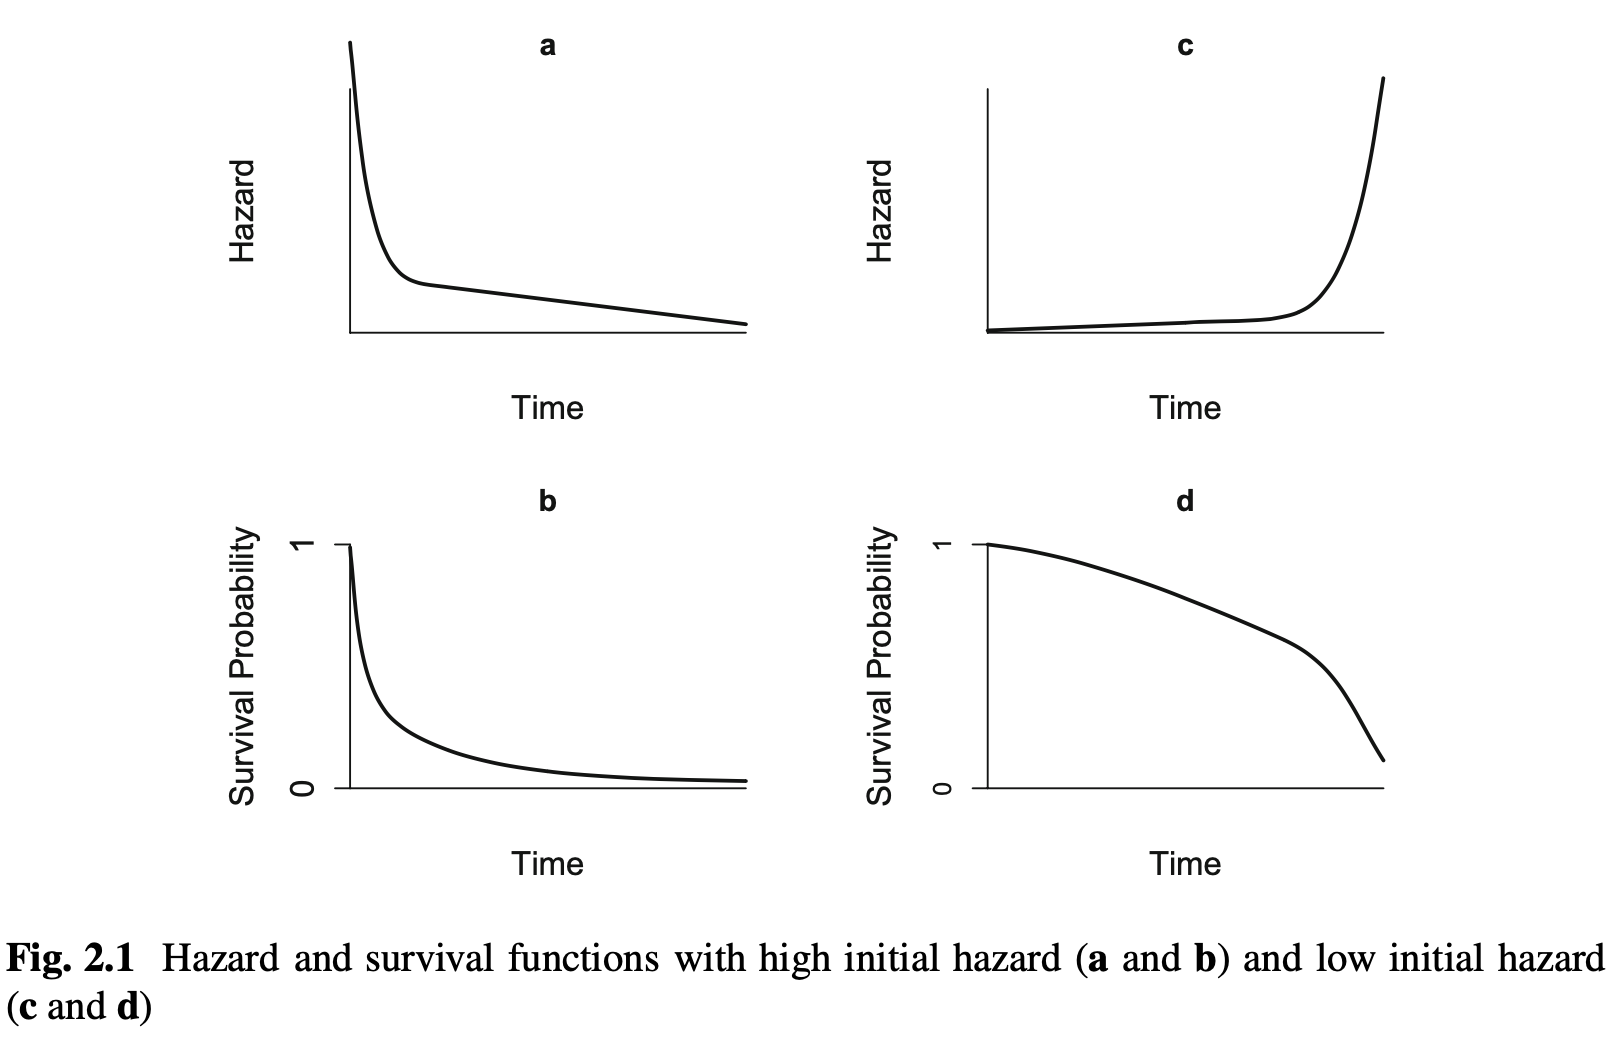
\includegraphics{images/hazard-01.png}
\caption{위험함수와 생존함수의 관계}
\end{figure}

생존함수와 위험함수는 다음과 같은 관계를 가지고 있다.

\begin{align*}
h(t) & = \frac{f(t)}{S(t)} \\
  & = \frac{f(t)}{1-F(t)} \\
  & = - \frac {\partial}{\partial t} \log [1-F(t)] \\
  & = - \frac {\partial}{\partial t} \log S(t)
\end{align*}

따라서 다음의 관계가 성립힌다.

\[ S(t) = exp[-H(t)] \]
여기서
\[ H(t) = \int_0^t h(t) dt \]
이며 \(H(t)\)를 누적 위험함수(cumulative hazard function)라고 한다.

위의 식에서 볼 수 있듯이 위험함수를 알면 생존함수를 쉽게 구할 수 있고 또한 반대로 생존함수를 알면 위험함수를 자동적으로 알게된다.

\hypertarget{uxc704uxd5d8uxd568uxc218uxc758-uxd615uxd0dc}{%
\section{위험함수의 형태}\label{uxc704uxd5d8uxd568uxc218uxc758-uxd615uxd0dc}}

앞에서 언급했듯이 위험함수는 시간에 따른 위험의 변화를 말해준다. 생존분석에서 중요한 분포들과 예제를 가지고 다양한 위험함수의 형태를 알아보자.

\begin{example}[지수분포]
\protect\hypertarget{exm:unnamed-chunk-3}{}{\label{exm:unnamed-chunk-3} \iffalse (지수분포) \fi{} }
만약 생존시간 \(T\)가 지수분포(Exponential distribution)을 따른다고 하자.

\[ f(t; \lambda) = \lambda e^{-\lambda t} \]

위에서 \(\lambda\) 는 흔히 단위시간 당 사망률, 실패율(failure rate)라고 부르며 \(E(T) = 1/\lambda\)이다.

생존함수(survaival function)와 위험함수(hazard function)은 다음과 같이 주어진다.

\begin{align*}
S(t) & = P(T>t)  = 1 - P(T \le t) \\
    & = 1 - \int_0^t \lambda e^{-\lambda t} \\
    & = 1 - (1-e^{-\lambda t} ) \\
    & = e^{-\lambda t} \\
h(t) & = \frac{f(t)}{S(t)} \\
    & = \lambda e^{-\lambda t}  / e^{-\lambda t} \\
    & = \lambda
\end{align*}

누적위험함수는 아래와 같다.
\[ H(t) = \int_0^t h(t) dt = \lambda t \]

생존시간이 지수분포를 따른다면 위험함수는 시간에 관계없이 상수 \(\lambda\)이다. 이렇게
시간에 따라서 위험함수가 상수인 경우는 현실에서는 거의 나타나지 않는다.
위험함수가 상수라는 것은 시간이 지나도 (1) 제품이 고정날 또는 (2) 사람이 사망할 위험성이 변허지 않는다는 의미이다.

지수분포는 생존분석에서 중요한 의미를 가진다. 즉, 생존시간이 지수분포를 따르면 개체는 얼마나 시간이 경과했는지 정보가 없다는 것이며 주어진 시각에 사건이 일어나지 않았다면 바로 다음 시간에 사건이 일어날
확률은 언제나 동일하다. \(\blacksquare\)
\end{example}

\begin{example}[와이블분포]
\protect\hypertarget{exm:unnamed-chunk-4}{}{\label{exm:unnamed-chunk-4} \iffalse (와이블분포) \fi{} }
만약 생존시간이 와이블 분포(Weibull distribution)를 따른다면 확률밀도함수는 다음과 같다.

\[ f(t) = \frac{\lambda t^{\lambda-1}}{\theta^\lambda}
\exp \left[ - \left(\frac{t}{\theta} \right)^\lambda \right],
\quad \theta,\lambda>0,  t \geq 0.
\]

평균은 \(E(T)=\theta \Gamma(1+1/\lambda)\) 이다. 여기서 \(\lambda=1\)이면 지수분포가 된다.

이때 생존 함수는 다음과 같다.
\begin{eqnarray*}
  S(t) &=& 1-\int_0^t \frac{\lambda t^{\lambda-1}}{\theta^\lambda} \exp \left[
- \left( \frac{t}{\theta} \right)^\lambda  \right] dt \\
 &=& \exp \left[
- \left( \frac{t}{\theta} \right)^\lambda  \right].
\end{eqnarray*}

또한 위험함수는 다음과 같다.
\begin{eqnarray*}
h(t) &=& \frac{f(t)}{S(t)} \\
   &=& \frac{\frac{\lambda t^{\lambda-1}}{\theta^\lambda} \exp \left[
- \left( \frac{t}{\theta} \right)^\lambda  \right]}{\exp \left[
- \left( \frac{t}{\theta} \right)^\lambda  \right]}  \\
   &=& \left( \frac{\lambda }{\theta^\lambda} \right) t^{\lambda-1}.
\end{eqnarray*}

위에서 볼 수 있듯이 \(\lambda=1\)이면 지수분포가 되고 위험함수는 상수이다. 만약에 \(\lambda>1\)이면
위험함수는 시간에 따라 증가하며 \(\lambda<1\)이면 위험함수는 감소한다.

누적위험함수는 아래와 같다.
\[ H(t) = \int_0^t h(t) dt = (t/\theta)^\lambda \]
\end{example}

다음은 모수의 변화에 따른 와이블 분포의 위험함수이다.

\begin{Shaded}
\begin{Highlighting}[]
\NormalTok{weibHaz }\OtherTok{\textless{}{-}}\NormalTok{ \{}\ControlFlowTok{function}\NormalTok{(x, shape, scale) }\FunctionTok{dweibull}\NormalTok{(x, }\AttributeTok{shape=}\NormalTok{shape,}
     \AttributeTok{scale=}\NormalTok{scale)}\SpecialCharTok{/}\FunctionTok{pweibull}\NormalTok{(x, }\AttributeTok{shape=}\NormalTok{shape, }\AttributeTok{scale=}\NormalTok{scale, }\AttributeTok{lower.tail=}\NormalTok{F)\}}
\FunctionTok{curve}\NormalTok{(}\FunctionTok{weibHaz}\NormalTok{(x, }\AttributeTok{shape=}\FloatTok{1.5}\NormalTok{, }\AttributeTok{scale=}\DecValTok{1}\SpecialCharTok{/}\FloatTok{0.03}\NormalTok{), }\AttributeTok{from=}\DecValTok{0}\NormalTok{, }\AttributeTok{to=}\DecValTok{80}\NormalTok{, }
     \AttributeTok{ylab=}\StringTok{\textquotesingle{}Hazard\textquotesingle{}}\NormalTok{, }\AttributeTok{xlab=}\StringTok{\textquotesingle{}Time\textquotesingle{}}\NormalTok{, }\AttributeTok{col=}\StringTok{"blue"}\NormalTok{)}
\FunctionTok{curve}\NormalTok{(}\FunctionTok{weibHaz}\NormalTok{(x, }\AttributeTok{shape=}\FloatTok{1.0}\NormalTok{, }\AttributeTok{scale=}\DecValTok{1}\SpecialCharTok{/}\FloatTok{0.03}\NormalTok{), }\AttributeTok{from=}\DecValTok{0}\NormalTok{, }\AttributeTok{to=}\DecValTok{80}\NormalTok{, }
     \AttributeTok{ylab=}\StringTok{\textquotesingle{}Hazard\textquotesingle{}}\NormalTok{, }\AttributeTok{xlab=}\StringTok{\textquotesingle{}Time\textquotesingle{}}\NormalTok{, }\AttributeTok{add=}\NormalTok{T, }\AttributeTok{col=}\StringTok{"black"}\NormalTok{)}
\FunctionTok{curve}\NormalTok{(}\FunctionTok{weibHaz}\NormalTok{(x, }\AttributeTok{shape=}\FloatTok{0.75}\NormalTok{, }\AttributeTok{scale=}\DecValTok{1}\SpecialCharTok{/}\FloatTok{0.03}\NormalTok{), }\AttributeTok{from=}\DecValTok{0}\NormalTok{, }\AttributeTok{to=}\DecValTok{80}\NormalTok{, }
     \AttributeTok{ylab=}\StringTok{\textquotesingle{}Hazard\textquotesingle{}}\NormalTok{, }\AttributeTok{xlab=}\StringTok{\textquotesingle{}Time\textquotesingle{}}\NormalTok{, }\AttributeTok{add=}\NormalTok{T, }\AttributeTok{col=}\StringTok{"red"}\NormalTok{)}
\FunctionTok{text}\NormalTok{(}\DecValTok{45}\NormalTok{, }\FloatTok{0.065}\NormalTok{, }\FunctionTok{expression}\NormalTok{(lambda }\SpecialCharTok{==} \FloatTok{1.50}\NormalTok{), }\AttributeTok{col=}\StringTok{"red"}\NormalTok{, }\AttributeTok{cex=}\FloatTok{1.3}\NormalTok{)}
\FunctionTok{text}\NormalTok{(}\DecValTok{58}\NormalTok{, }\FloatTok{0.065}\NormalTok{, }\FunctionTok{expression}\NormalTok{(theta}\SpecialCharTok{==}\DecValTok{1}\SpecialCharTok{/}\FloatTok{0.03}\NormalTok{), }\AttributeTok{col=}\StringTok{"red"}\NormalTok{, }\AttributeTok{cex=}\FloatTok{1.3}\NormalTok{)}
\FunctionTok{text}\NormalTok{(}\DecValTok{45}\NormalTok{, }\FloatTok{0.015}\NormalTok{, }\FunctionTok{expression}\NormalTok{(lambda }\SpecialCharTok{==} \FloatTok{0.75}\NormalTok{), }\AttributeTok{col=}\StringTok{"blue"}\NormalTok{, }\AttributeTok{cex=}\FloatTok{1.3}\NormalTok{)}
\FunctionTok{text}\NormalTok{(}\DecValTok{58}\NormalTok{, }\FloatTok{0.015}\NormalTok{, }\FunctionTok{expression}\NormalTok{(theta}\SpecialCharTok{==}\DecValTok{1}\SpecialCharTok{/}\FloatTok{0.03}\NormalTok{), }\AttributeTok{col=}\StringTok{"blue"}\NormalTok{, }\AttributeTok{cex=}\FloatTok{1.3}\NormalTok{)}
\FunctionTok{text}\NormalTok{(}\DecValTok{45}\NormalTok{, }\FloatTok{0.034}\NormalTok{, }\FunctionTok{expression}\NormalTok{(lambda}\SpecialCharTok{==} \FloatTok{1.00}\NormalTok{), }\AttributeTok{col=}\StringTok{"black"}\NormalTok{, }\AttributeTok{cex=}\FloatTok{1.3}\NormalTok{)}
\FunctionTok{text}\NormalTok{(}\DecValTok{58}\NormalTok{, }\FloatTok{0.034}\NormalTok{, }\FunctionTok{expression}\NormalTok{(theta}\SpecialCharTok{==}\DecValTok{1}\SpecialCharTok{/}\FloatTok{0.03}\NormalTok{), }\AttributeTok{col=}\StringTok{"black"}\NormalTok{, }\AttributeTok{cex=}\FloatTok{1.3}\NormalTok{)}
\end{Highlighting}
\end{Shaded}

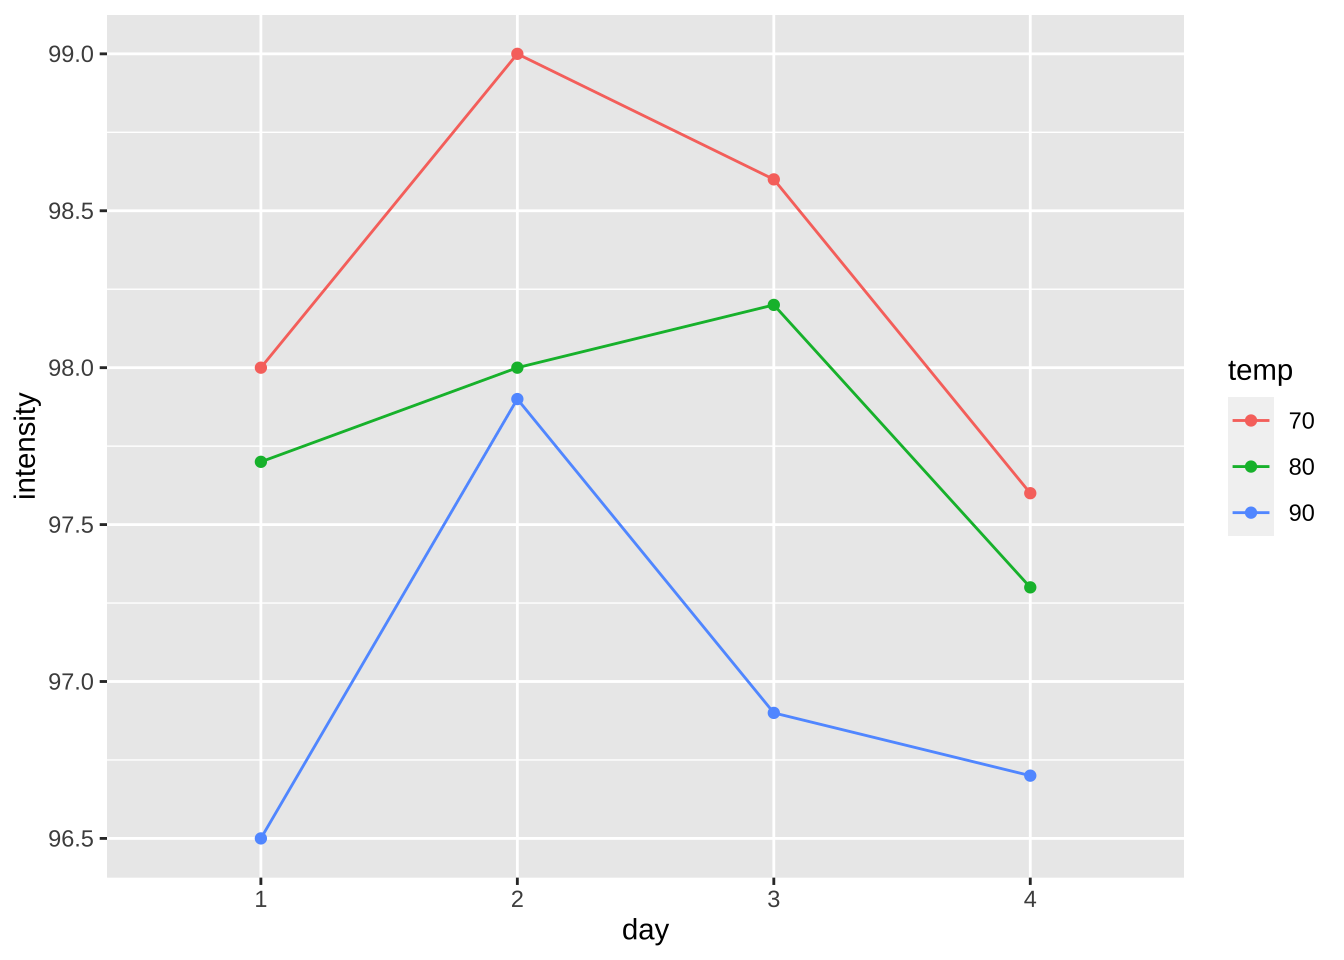
\includegraphics{survival_files/figure-latex/unnamed-chunk-5-1.pdf}

\(\blacksquare\)

\begin{example}[미국 여자와 남자의 연령에 따른 사망위험율]
\protect\hypertarget{exm:unnamed-chunk-6}{}{\label{exm:unnamed-chunk-6} \iffalse (미국 여자와 남자의 연령에 따른 사망위험율) \fi{} }
다음 그림은 미국 여자와 남자의 연령에 따른 사망위험율을 나타내는 위험함수를 보여주는 그림이다.
Y 축은 로그 스케일로 그린 그림이며 2004년의 자료를 이용하여 그린 그림이다.
태어난 날과 그 후 몇 주동안은 매우 사망위험이 높다가 급격하게 떨어진다. 그리고 10대에서 약간의 증가 현상을 보이며 조금 감쏘하다가 시간이 지날수록 위험율이 완만하게 증가한다. 주목할 점은 남자가 여자보다 사망의 위험이 언제나 크다는 것이며 이는 잘 알려진 사실이다.
\end{example}

\begin{Shaded}
\begin{Highlighting}[]
\NormalTok{tm }\OtherTok{\textless{}{-}} \FunctionTok{c}\NormalTok{(}\DecValTok{0}\NormalTok{, }\CommentTok{\# birth}
   \DecValTok{1}\SpecialCharTok{/}\DecValTok{365}\NormalTok{, }\CommentTok{\# first day of life}
   \DecValTok{7}\SpecialCharTok{/}\DecValTok{365}\NormalTok{, }\CommentTok{\# seventh day of life}
   \DecValTok{28}\SpecialCharTok{/}\DecValTok{365}\NormalTok{, }\CommentTok{\# fourth week of life}
   \DecValTok{1}\SpecialCharTok{:}\DecValTok{107}\NormalTok{) }\CommentTok{\# subsequent years}
\NormalTok{hazMale }\OtherTok{\textless{}{-}} \FunctionTok{as.numeric}\NormalTok{(survexp.us[,}\StringTok{"male"}\NormalTok{,}\StringTok{"2004"}\NormalTok{]) }\CommentTok{\# 2004 males}
\NormalTok{hazFemale }\OtherTok{\textless{}{-}} \FunctionTok{as.numeric}\NormalTok{(survexp.us[,}\StringTok{"female"}\NormalTok{,}\StringTok{"2004"}\NormalTok{]) }\CommentTok{\# 2004 females}
\NormalTok{tm.diff }\OtherTok{\textless{}{-}} \FunctionTok{diff}\NormalTok{(tm)}
\NormalTok{survMale }\OtherTok{\textless{}{-}} \FunctionTok{exp}\NormalTok{(}\SpecialCharTok{{-}}\FunctionTok{cumsum}\NormalTok{(hazMale}\SpecialCharTok{*}\NormalTok{tm.diff)}\SpecialCharTok{*}\FloatTok{365.24}\NormalTok{)}
\NormalTok{survFemale }\OtherTok{\textless{}{-}} \FunctionTok{exp}\NormalTok{(}\SpecialCharTok{{-}}\FunctionTok{cumsum}\NormalTok{(hazFemale}\SpecialCharTok{*}\NormalTok{tm.diff)}\SpecialCharTok{*}\FloatTok{365.24}\NormalTok{)}

\CommentTok{\# Figure 2.1.2 log hazard and survival for US males and females in 2004}
\FunctionTok{par}\NormalTok{(}\AttributeTok{mfrow=}\FunctionTok{c}\NormalTok{(}\DecValTok{2}\NormalTok{,}\DecValTok{1}\NormalTok{),    }\CommentTok{\# two rows and one column of plots}
    \AttributeTok{mar=}\FunctionTok{c}\NormalTok{(}\FloatTok{4.2}\NormalTok{,}\DecValTok{5}\NormalTok{,}\DecValTok{2}\NormalTok{,}\DecValTok{2}\NormalTok{))  }\CommentTok{\# set margins for the lower, left, top, and righ of each plot}

\NormalTok{logHazMale }\OtherTok{\textless{}{-}} \FunctionTok{log}\NormalTok{(hazMale)}
\NormalTok{logHazFemale }\OtherTok{\textless{}{-}} \FunctionTok{log}\NormalTok{(hazFemale)    }

\FunctionTok{plot}\NormalTok{(logHazMale }\SpecialCharTok{\textasciitilde{}}\NormalTok{ tm[}\SpecialCharTok{{-}}\DecValTok{1}\NormalTok{], }\AttributeTok{type=}\StringTok{"l"}\NormalTok{,}
     \AttributeTok{xlab=}\StringTok{"Age in years"}\NormalTok{,           }\CommentTok{\# x axis label}
     \AttributeTok{ylab=}\StringTok{"Hazard"}\NormalTok{,}\AttributeTok{col=}\StringTok{"blue"}\NormalTok{,      }\CommentTok{\# y azis label}
     \AttributeTok{lwd=}\DecValTok{2}\NormalTok{,                         }\CommentTok{\# double line width}
     \AttributeTok{las=}\DecValTok{1}\NormalTok{,                         }\CommentTok{\# make y axis labels perpendicular to axis}
     \AttributeTok{axes=}\NormalTok{F, }\AttributeTok{cex.lab=}\FloatTok{1.3}\NormalTok{, }\AttributeTok{cex.axis=}\FloatTok{1.3}\NormalTok{)     }\CommentTok{\# make blue line solid}
\FunctionTok{lines}\NormalTok{(logHazFemale }\SpecialCharTok{\textasciitilde{}}\NormalTok{ tm[}\SpecialCharTok{{-}}\DecValTok{1}\NormalTok{],}\AttributeTok{type=}\StringTok{"l"}\NormalTok{, }
      \AttributeTok{col=}\StringTok{"red"}\NormalTok{,}\AttributeTok{lwd=}\DecValTok{2}\NormalTok{, }\AttributeTok{lty=}\DecValTok{2}\NormalTok{)   }\CommentTok{\# add a red dashed line to the plot}

\NormalTok{yyLabs }\OtherTok{\textless{}{-}} \FunctionTok{c}\NormalTok{(}\FloatTok{1e{-}07}\NormalTok{, }\FloatTok{1e{-}06}\NormalTok{, }\FloatTok{1e{-}05}\NormalTok{, }\FloatTok{1e{-}04}\NormalTok{, }\FloatTok{1e{-}03}\NormalTok{, }\FloatTok{1e{-}02}\NormalTok{)}
\NormalTok{yyLabsLog }\OtherTok{\textless{}{-}} \FunctionTok{log}\NormalTok{(yyLabs)}
\FunctionTok{axis}\NormalTok{(}\DecValTok{2}\NormalTok{, }\AttributeTok{at=}\NormalTok{yyLabsLog, }\AttributeTok{labels=}\FunctionTok{c}\NormalTok{(}\FunctionTok{expression}\NormalTok{(}\DecValTok{10}\SpecialCharTok{\^{}{-}}\DecValTok{7}\NormalTok{), }\FunctionTok{expression}\NormalTok{(}\DecValTok{10}\SpecialCharTok{\^{}{-}}\DecValTok{6}\NormalTok{), }
  \FunctionTok{expression}\NormalTok{(}\DecValTok{10}\SpecialCharTok{\^{}{-}}\DecValTok{5}\NormalTok{), }\FunctionTok{expression}\NormalTok{(}\DecValTok{10}\SpecialCharTok{\^{}{-}}\DecValTok{4}\NormalTok{), }\FunctionTok{expression}\NormalTok{(}\DecValTok{10}\SpecialCharTok{\^{}{-}}\DecValTok{3}\NormalTok{), }\FunctionTok{expression}\NormalTok{(}\DecValTok{10}\SpecialCharTok{\^{}{-}}\DecValTok{2}\NormalTok{)), }\AttributeTok{las=}\DecValTok{1}\NormalTok{)  }
\FunctionTok{axis}\NormalTok{(}\DecValTok{1}\NormalTok{, }\AttributeTok{cex.axis=}\FloatTok{1.3}\NormalTok{)   }
\FunctionTok{legend}\NormalTok{(}\StringTok{"bottomright"}\NormalTok{, }\AttributeTok{legend=}\FunctionTok{c}\NormalTok{(}\StringTok{"males"}\NormalTok{,}\StringTok{"females"}\NormalTok{),}
       \AttributeTok{lty=}\FunctionTok{c}\NormalTok{(}\DecValTok{1}\NormalTok{,}\DecValTok{2}\NormalTok{), }\AttributeTok{col=}\FunctionTok{c}\NormalTok{(}\StringTok{"blue"}\NormalTok{,}\StringTok{"red"}\NormalTok{), }\AttributeTok{lwd=}\DecValTok{2}\NormalTok{, }\AttributeTok{cex=}\FloatTok{1.3}\NormalTok{)}
\FunctionTok{title}\NormalTok{(}\StringTok{"Hazards for US males and females in 2004"}\NormalTok{)}

\NormalTok{tm.diff }\OtherTok{\textless{}{-}} \FunctionTok{diff}\NormalTok{(tm)         }\CommentTok{\# same length as "tm"}
\NormalTok{survMale }\OtherTok{\textless{}{-}} \FunctionTok{exp}\NormalTok{(}\SpecialCharTok{{-}}\FunctionTok{cumsum}\NormalTok{(hazMale}\SpecialCharTok{*}\NormalTok{tm.diff)}\SpecialCharTok{*}\FloatTok{365.24}\NormalTok{)         }\CommentTok{\# survival probs for males}
\NormalTok{survFemale }\OtherTok{\textless{}{-}} \FunctionTok{exp}\NormalTok{(}\SpecialCharTok{{-}}\FunctionTok{cumsum}\NormalTok{(hazFemale}\SpecialCharTok{*}\NormalTok{tm.diff)}\SpecialCharTok{*}\FloatTok{365.24}\NormalTok{)     }\CommentTok{\# survival probs for females}
\CommentTok{\#windows(width=7,height=5)}
\FunctionTok{plot}\NormalTok{(survMale }\SpecialCharTok{\textasciitilde{}}\NormalTok{ tm[}\SpecialCharTok{{-}}\DecValTok{1}\NormalTok{],}\AttributeTok{type=}\StringTok{"l"}\NormalTok{,          }\CommentTok{\# lower case "L" indicates line plot}
     \AttributeTok{xlab=}\StringTok{"Age in years"}\NormalTok{,             }\CommentTok{\# x axis label}
     \AttributeTok{ylab=}\StringTok{"Survival probability"}\NormalTok{,     }\CommentTok{\# y azis label}
     \AttributeTok{col=}\StringTok{"blue"}\NormalTok{,                      }\CommentTok{\# line color}
     \AttributeTok{lwd=}\DecValTok{2}\NormalTok{,                           }\CommentTok{\# double line width}
     \AttributeTok{las=}\DecValTok{1}\NormalTok{,                           }\CommentTok{\# make y axis labels perpendicular to axis}
     \AttributeTok{ylim=}\FunctionTok{c}\NormalTok{(}\DecValTok{0}\NormalTok{,}\DecValTok{1}\NormalTok{), }\AttributeTok{cex.lab=}\FloatTok{1.3}\NormalTok{, }\AttributeTok{cex.axis=}\FloatTok{1.3}\NormalTok{)       }\CommentTok{\# y axis limit ranges from 0 to 1}

\FunctionTok{lines}\NormalTok{(survFemale }\SpecialCharTok{\textasciitilde{}}\NormalTok{ tm[}\SpecialCharTok{{-}}\DecValTok{1}\NormalTok{], }\AttributeTok{col=}\StringTok{"red"}\NormalTok{, }\AttributeTok{lwd=}\DecValTok{2}\NormalTok{, }\AttributeTok{lty=}\DecValTok{2}\NormalTok{)    }\CommentTok{\# add a red dashed line to the plot}
\FunctionTok{legend}\NormalTok{(}\StringTok{"bottomleft"}\NormalTok{, }\AttributeTok{legend=}\FunctionTok{c}\NormalTok{(}\StringTok{"males"}\NormalTok{,}\StringTok{"females"}\NormalTok{),}
       \AttributeTok{lty=}\FunctionTok{c}\NormalTok{(}\DecValTok{1}\NormalTok{,}\DecValTok{2}\NormalTok{), }\AttributeTok{col=}\FunctionTok{c}\NormalTok{(}\StringTok{"blue"}\NormalTok{,}\StringTok{"red"}\NormalTok{), }\AttributeTok{lwd=}\DecValTok{2}\NormalTok{, }\AttributeTok{cex=}\FloatTok{1.3}\NormalTok{)}
\FunctionTok{title}\NormalTok{(}\StringTok{"Survival of US males and females in 2004"}\NormalTok{)}
\end{Highlighting}
\end{Shaded}

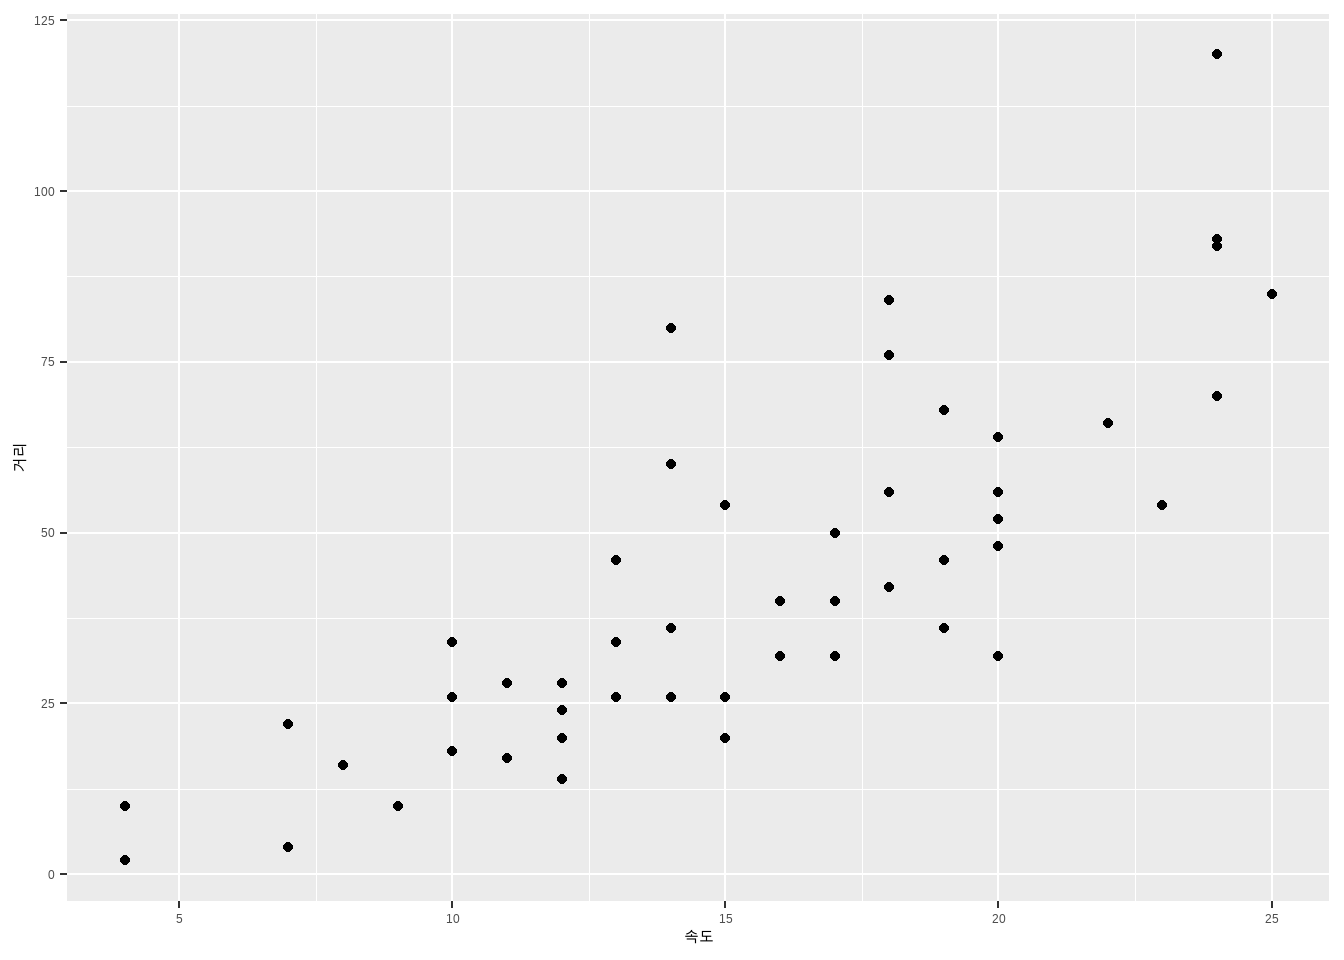
\includegraphics{survival_files/figure-latex/unnamed-chunk-7-1.pdf}

\(\blacksquare\)

\hypertarget{uxd3c9uxade0-uxc0dduxc874uxc2dcuxac04uxacfc-uxc911uxc704-uxc0dduxc874uxc2dcuxac04}{%
\section{평균 생존시간과 중위 생존시간}\label{uxd3c9uxade0-uxc0dduxc874uxc2dcuxac04uxacfc-uxc911uxc704-uxc0dduxc874uxc2dcuxac04}}

평균 생존시간 \(\mu\) 다은과 같이 정의된다.

\[ \mu = \int_{0}^\infty t f(t) dt \]

잘 알려진 생존함수의 공식 \(f(t) = dS(t)/dt\)와 부분 적분 공식(integration by part)를 이용하면\\
평균 생존시간 \(\mu\) 다은과 같이 구할 수 있다.

\[ \mu = \int_0^\infty S(t)dt \]
중위 생존시간은 \(t_{med}\) 다음 방정식을 만족하는 \(t\)의 값이다.

\[ t_{med} = \inf ~ \{t~|~ S(t) \le 1/2 \} \]

\hypertarget{uxc784uxc758uxc911uxb3c4uxc808uxb2e8}{%
\section{임의중도절단}\label{uxc784uxc758uxc911uxb3c4uxc808uxb2e8}}

\begin{figure}
\centering
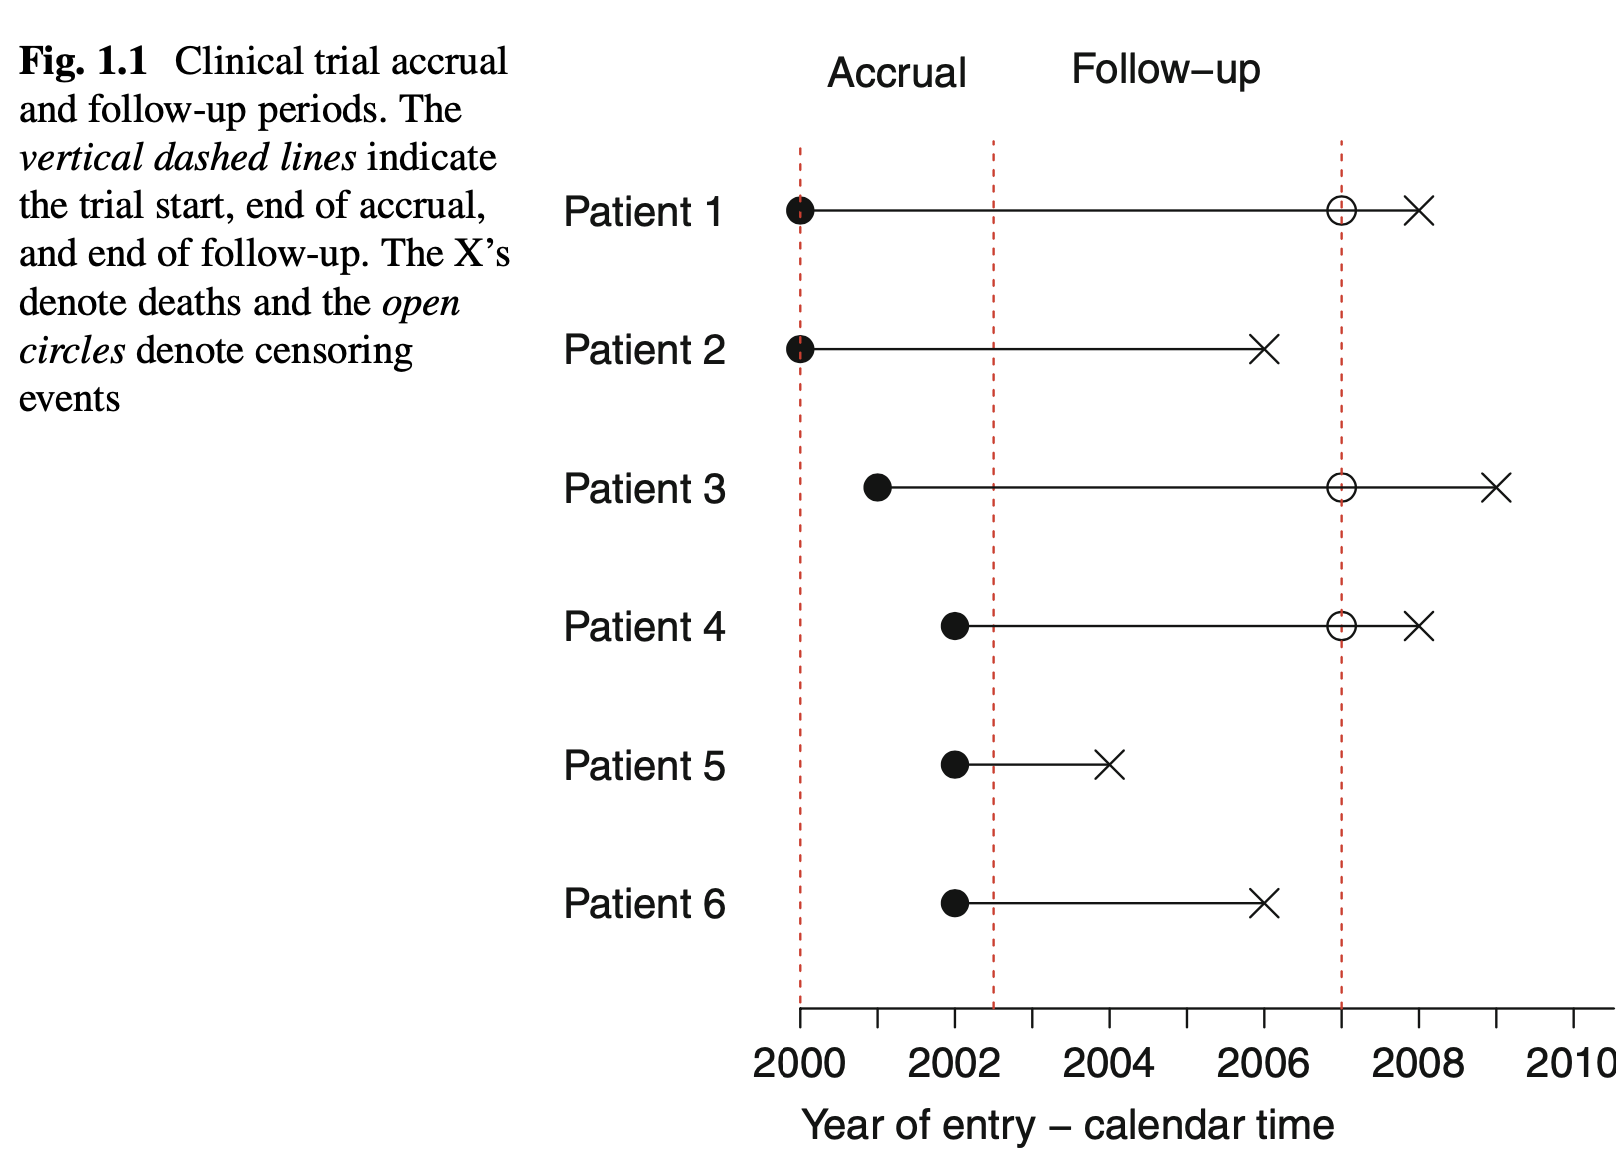
\includegraphics{images/censoring.png}
\caption{중도 절단 자료}
\end{figure}

생존시간 \(T_1, T_2, \dots, T_n\)을 독립적으로 분포 \(f_\theta(t)\)에서 추출하였다고 가정하고 중도절단시간
\(C_1, C_2, \dots, C_n\)도 독립적으로 분포 \(g(c)\)에서 추출하였다고 가정하자.

생존시간 \(T\)와 중도절단시간 \(C\)가 서로 독립이라고 가정하며 이러한 가정을 임의 중도절단(random censoring)이라고 한다.

이제 관측한 생존시간 \(X_i\)는 다음과 같이 정의한다.

\[ X_i = \min (T_i, C_i) \quad i=1,2,\dots, n \]

또한 절단 표시변수 \(\delta_i\)는 다음과 같이 정의한다. 표시변수 \(\delta_i\) 가 1의 값을 가지면
실제 생존시간을 관측한 것이고 0이면 절단된 자료이다.

\[ \delta_i = \begin{cases}
1 & T_i < C_i \\
0 & T_i > C_i 
\end{cases} \]

따라서 중도절단이 있는 자료는 다음과 같은 각 개체에 대한여 쌍으로 구성된 관측값이 얻어진다.

\[ (X_1, \delta_1), (X_2, \delta_2), \dots, (X_n, \delta_n) \]

\hypertarget{uxbaa8uxc218uxc758-uxcd5cuxb300uxac00uxb2a5uxb3c4-uxcd94uxc815}{%
\section{모수의 최대가능도 추정}\label{uxbaa8uxc218uxc758-uxcd5cuxb300uxac00uxb2a5uxb3c4-uxcd94uxc815}}

이제 생존시간 \(T\)의 분포 \(F_\theta(t)\) 가 주어졌을 때 표본 \((x_i, \delta_i)\)의 가능도 함수 \(L\) 는 다음과 같이 나타낼 수 있다.

\[ L(\theta; x, \delta) = \prod_{i \in UC} P_\theta(T_i= x_i ) \prod_{i \in C} P_\theta(T_i > x_i ) = \prod_{i \in UC} f_\theta( x_i ) \prod_{i \in C} [1-F_\theta( x_i )] \]

여기서 집합 \(UC\)는 실제 생존시간이 관측된 자료들, 집합 \(C\)는 중도절단된 자료을 의미한다.

모수의 최대가능도 추정은 \(L(\theta; X, \delta)\)를 최대로 하는 \(\theta\)를 찾는 방법이다.

이제 예제로서 생존시간의 분포가 지수분포를 따른다고 가정하고 가능도함수를 구해보자.

\begin{align*}
L(\lambda; x, \delta) & = \prod_{i \in UC} P_\lambda(T_i= x_i ) \prod_{i \in C} P_\lambda(T_i > x_i ) \\
  & = \prod_{i \in UC} f_\lambda( x_i ) \prod_{i \in C} [1-F_\lambda( x_i )] \\
  & = \prod_{i=1}^n \left [ \lambda e^{-\lambda x_i} \right ]^{\delta_i} \left [e^{-\lambda x_i} \right ]^{1-\delta_i} \\
  & = \prod_{i=1}^n \lambda^{\delta_i} e^{-\lambda x_i} \\
  & = \lambda^{ \sum_{i=1}^n \delta_i} e^{-\lambda \sum_{i=1}^n x_i} 
\end{align*}

이제 위의 가능도함수를 최대화하는 모수를 찾기위하여 로그가능도함수를 고려하고

\[ \ell (\lambda; x, \delta) = \log L(\lambda; x, \delta) = 
    \log \lambda \sum_{i=1}^n \delta_i - \lambda \sum_{i=1}^n x_i \]

로그가능도함수를 모수 \(\lambda\)에 대하여 미분하고 0으로 놓고 풀면 최대가능도 추정량을 구할 수 있다.

\[ \frac{\partial}{\partial \lambda} \ell (\lambda; x, \delta) = 
     \frac{\sum_{i=1}^n \delta_i}{\lambda} - \sum_{i=1}^n x_i = 0 \]
따라서 최대가능도 추정량은 다음과 같이 주어진다.
\[ \hat \lambda_{ML} = \frac{\sum_{i=1}^n \delta_i}{\sum_{i=1}^n x_i} \]

만약 중도절단자료가 없다면 최대가능도 추정량은 일반적인 경우와 같이 다음과 같다.

\[ \hat \lambda_{ML} = \frac{n}{\sum_{i=1}^n x_i} \]

\hypertarget{estsurvival}{%
\chapter{생존함수의 추정}\label{estsurvival}}

\hypertarget{uxc0dduxba85uxd45cuxbc29uxbc95uxc744-uxc774uxc6a9uxd55c-uxc0dduxc874uxd568uxc218-uxcd94uxc815}{%
\section{생명표방법을 이용한 생존함수 추정}\label{uxc0dduxba85uxd45cuxbc29uxbc95uxc744-uxc774uxc6a9uxd55c-uxc0dduxc874uxd568uxc218-uxcd94uxc815}}

시간 \((0, \infty)\)구간을 다음과 같은 경계선을 이용하여 \(k+1\) 개의 구간으로 나누었다고 가정하자. (\(t_0=0\))

\[ (t_0, t_1] \quad (t_1,t_2] \quad \dots \quad (t_{k-1}, t_k] \quad (t_k, \infty) \]

생존함수는 다음과 같은 조건부 확률의 축차식으로 구할 수 있다.

\begin{align*}
S(t_i) & = p(T>t_i) \\
    & = P(T > t_i | T > t_{i-1}) P(T > t_{i-1}) \\
    & = P(T > t_i | T > t_{i-1}) P(T > t_{i-1} | T > t_{i-2}) P(T > t_{i-2} )  \\
    & = \cdots \\
    & = P(T > t_i | T > t_{i-1}) P(T > t_{i-1} | T > t_{i-2}) P(T > t_{i-2} )  \dots  P(T> t_2 | T > t_1)P(T > t_1)
\end{align*}

생명표방법을 이용한 생존함수 추정은 표를 이용하면 편리하다. 다음은 표를 생명표방법을 이용하여 생존함수를 추정하는 예를 보여준다.

\begin{longtable}[]{@{}llllllll@{}}
\toprule
구간 & 위험그룹인원수 & 사망자 수 & 중도절단 수 & 유효인원수 & 사망율 & 생존율 & 생존함수 추정\tabularnewline
\midrule
\endhead
\(I_i\) & \(n_i\) & \(d_i\) & \(c_i\) & \(n'_i\) & \(\tfrac{d_i}{n'_i}\) & \(1-\tfrac{d_i}{n'_i}\) & \(\hat S(t_i)\)\tabularnewline
0-1 & 126 & 47 & 19 & 116.5 & 0.40 & 0.60 & 0.60\tabularnewline
1-2 & 60 & 5 & 17 & 51.5 & 0.10 & 0.90 & 0.54\tabularnewline
2-3 & 38 & 2 & 15 & 30.5 & 0.07 & 0.93 & 0.50\tabularnewline
3-4 & 21 & 2 & 9 & 16.5 & 0.12 & 0.88 & 0.44\tabularnewline
4-5 & 10 & 0 & 6 & 7.0 & 0.00 & 1.00 & 0.44\tabularnewline
\bottomrule
\end{longtable}

위에서 유효인원수는 다음과 같이 계산한다.

\[ n'_i = n_i - \frac{c_i}{2} \]

또한 생존함수의 추정식은는 조건부 확률의 축차식을 이용하여 다음과 같이 계산한다.

\[ \hat S(t_i) = \prod_{k=1}^i \hat p_k = \prod_{k=1}^i  \left ( 1-\tfrac{d_k}{n'_k} \right ) \]

이와 같이 주정된 생존함수의 분산은 다음과 같은 그린우드의 공식으로 구할 수 있다.

\[ \widehat {Var} (\hat S (t_i) ) =  \hat S(t_i)  \sum_{k=1}^i \frac{d_k}{ n_k^{'} ( n_k^{'} -d_k)} \]

\hypertarget{uxb204uxc801uxd55cuxacc4uxcd94uxc815uxbc95uxc5d0-uxc758uxd55c-uxc0dduxc874uxd568uxc218-uxcd94uxc815}{%
\section{누적한계추정법에 의한 생존함수 추정}\label{uxb204uxc801uxd55cuxacc4uxcd94uxc815uxbc95uxc5d0-uxc758uxd55c-uxc0dduxc874uxd568uxc218-uxcd94uxc815}}

표본으로 추출한 생존시간들을 순서대로 \(t_1 < t_2 < \dots < t_n\) 나열한 다음 누적한계추정법은 생존함수를 다음의 식으로 추정한다.

\[ \hat S(t) =  \prod_{t_i \le t}  \left ( 1-\frac{d_i}{n_i} \right)^{\delta_i}
=  \prod_{t_i \le t}  \left ( \frac{n_i-d_k}{n_i} \right)^{\delta_i}\]

\begin{itemize}
\tightlist
\item
  \(n_i\) : 시간 \(t_i\) 바로 직전까지 중도절단되지 않고 생존한 사람의 수
\item
  \(d_i\) : 시간 \(t_i\) 에 사망한 사람의 수
\end{itemize}

생존함수 추정량 \(\hat S(t)\) 의 분산은 다음과 같이 주어진다.

\[ Var(\hat S(t)) = [\hat S(t)]^2 \sum_{t_i \le t} \frac{d_i}{n_i(n_i-d_i)} \]

위의 분산추정량으로 생존함수의 신뢰구간을 구하면 {[}0,1{]}의 범위를 벗어나는 경우가 생긴다. 이러한 단범을 보완하기 위하여 생존함수의 변환(log-log transformation)에 대한 신뢰구간을 구하는 방법을 주로 사용한다.

\[ Var\left ( \log \left [ - \log \hat S(t) \right ] \right )
\approx \frac{1}{[\hat S(t)]^2  } \sum_{t_i \le t} \frac{d_i}{n_i(n_i-d_i)} \]

\begin{example}[누적한계추정법]
\protect\hypertarget{exm:unnamed-chunk-8}{}{\label{exm:unnamed-chunk-8} \iffalse (누적한계추정법) \fi{} }다음 주어진 자료로부터 생존함수를 추정하는 방법을 알아보자. \(+\)는 중도절단된 자료를 표시한다.

\[ 9,~~13,~~13+,~~18,~~23~~,28+,~~31,~~,34,~~,45+,~~,48,~~161+ \]

누적한계추정법은 생존함수를 다음과 같이 축차적으로 구할 수 있다.
\end{example}

\begin{align*}
\hat S(0) & = 1 \\
\hat S(9) & = \hat S(0) \times \frac{10}{11} = 0.91 \\
\hat S(13) & = \hat S(9) \times \frac{9}{10} = 0.82 \\
\hat S(18) & = \hat S(13) \times \frac{7}{8} = 0.72 \\
\hat S(23) & = \hat S(18) \times \frac{6}{7} = 0.61 \\
\hat S(31) & = \hat S(23) \times \frac{4}{5} = 0.49 \\
\hat S(34) & = \hat S(31) \times \frac{3}{4} = 0.37 \\
\hat S(48) & = \hat S(34) \times \frac{1}{2} = 0.18 
\end{align*}

\(\blacksquare\)

다음은 예제 자료에 대하여 누적한계추정법으로 생존함수를 추정하는
R 프로그램이다.

\begin{Shaded}
\begin{Highlighting}[]
\NormalTok{t }\OtherTok{\textless{}{-}} \FunctionTok{c}\NormalTok{(}\DecValTok{9}\NormalTok{, }\DecValTok{13}\NormalTok{, }\DecValTok{13}\NormalTok{, }\DecValTok{18}\NormalTok{ ,}\DecValTok{23}\NormalTok{ ,}\DecValTok{28}\NormalTok{, }\DecValTok{31}\NormalTok{, }\DecValTok{34}\NormalTok{ ,}\DecValTok{45}\NormalTok{ ,}\DecValTok{48}\NormalTok{ ,}\DecValTok{161}\NormalTok{) }
\NormalTok{cens }\OtherTok{\textless{}{-}} \FunctionTok{c}\NormalTok{(}\DecValTok{1}\NormalTok{,}\DecValTok{1}\NormalTok{,}\DecValTok{0}\NormalTok{,}\DecValTok{1}\NormalTok{,}\DecValTok{1}\NormalTok{,}\DecValTok{0}\NormalTok{,}\DecValTok{1}\NormalTok{,}\DecValTok{1}\NormalTok{,}\DecValTok{0}\NormalTok{,}\DecValTok{1}\NormalTok{,}\DecValTok{0}\NormalTok{)}
\NormalTok{df }\OtherTok{\textless{}{-}} \FunctionTok{Surv}\NormalTok{(t, cens)}
\NormalTok{df}
\end{Highlighting}
\end{Shaded}

\begin{verbatim}
##  [1]   9   13   13+  18   23   28+  31   34   45+  48  161+
\end{verbatim}

\begin{Shaded}
\begin{Highlighting}[]
\NormalTok{res.km }\OtherTok{\textless{}{-}} \FunctionTok{survfit}\NormalTok{(}\FunctionTok{Surv}\NormalTok{(t, cens)}\SpecialCharTok{\textasciitilde{}}\DecValTok{1}\NormalTok{,  }\AttributeTok{conf.type=}\StringTok{"log{-}log"}\NormalTok{)}
\NormalTok{res.km}
\end{Highlighting}
\end{Shaded}

\begin{verbatim}
## Call: survfit(formula = Surv(t, cens) ~ 1, conf.type = "log-log")
## 
##       n  events  median 0.95LCL 0.95UCL 
##      11       7      31      13      NA
\end{verbatim}

\begin{Shaded}
\begin{Highlighting}[]
\FunctionTok{summary}\NormalTok{(res.km)}
\end{Highlighting}
\end{Shaded}

\begin{verbatim}
## Call: survfit(formula = Surv(t, cens) ~ 1, conf.type = "log-log")
## 
##  time n.risk n.event survival std.err lower 95% CI upper 95% CI
##     9     11       1    0.909  0.0867       0.5081        0.987
##    13     10       1    0.818  0.1163       0.4474        0.951
##    18      8       1    0.716  0.1397       0.3502        0.899
##    23      7       1    0.614  0.1526       0.2658        0.835
##    31      5       1    0.491  0.1642       0.1673        0.753
##    34      4       1    0.368  0.1627       0.0928        0.657
##    48      2       1    0.184  0.1535       0.0117        0.525
\end{verbatim}

\begin{Shaded}
\begin{Highlighting}[]
\FunctionTok{plot}\NormalTok{(res.km)}
\end{Highlighting}
\end{Shaded}

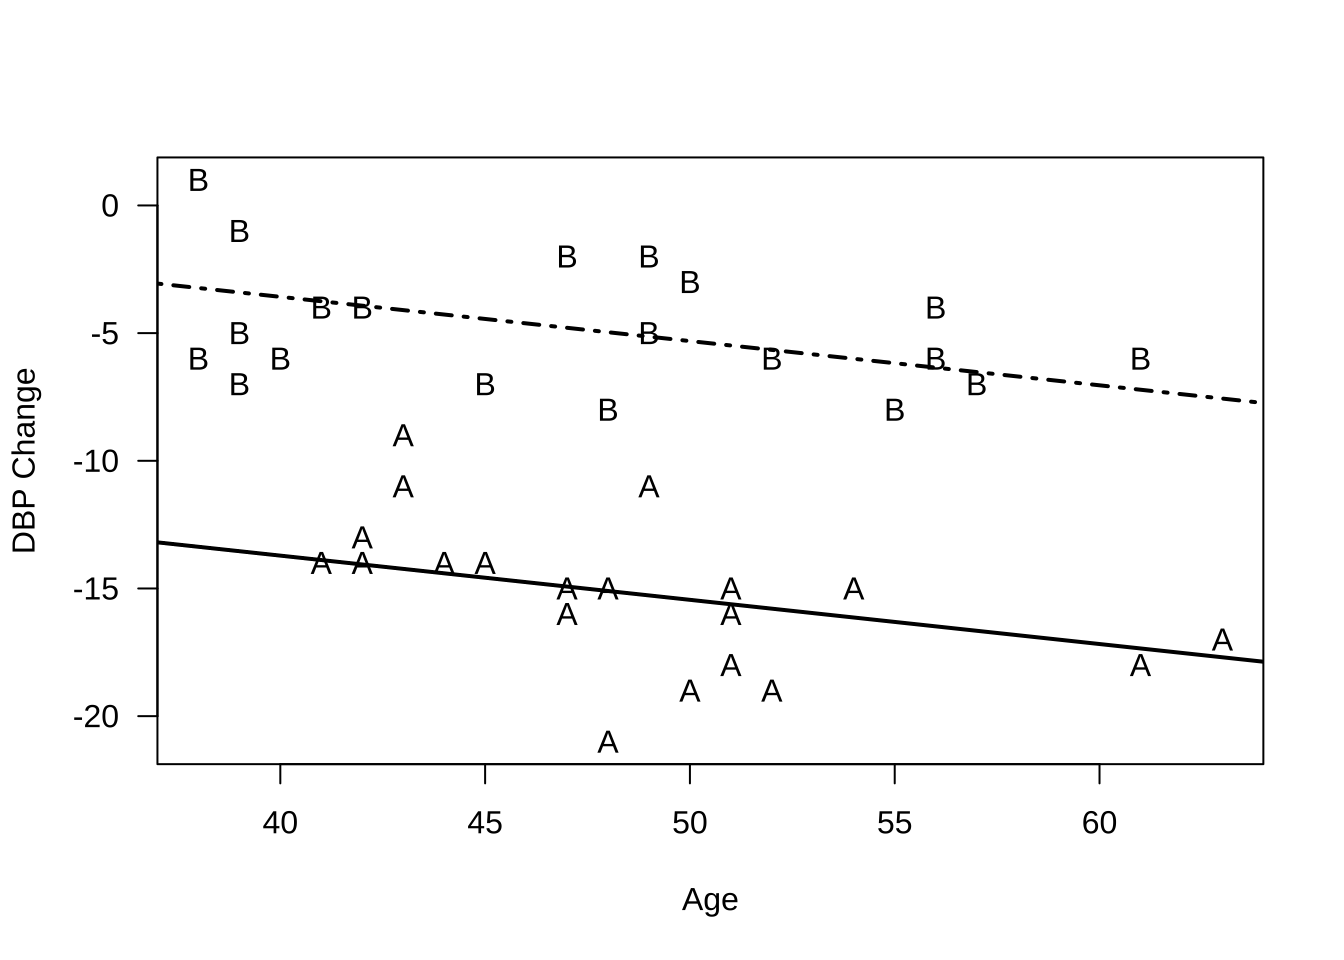
\includegraphics{survival_files/figure-latex/unnamed-chunk-9-1.pdf}

\hypertarget{nelson-aalen-uxcd94uxc815uxb7c9}{%
\section{Nelson-Aalen 추정량}\label{nelson-aalen-uxcd94uxc815uxb7c9}}

Nelson-Aalen 추정량은 생존함수와 위험함수의 관계를 이용하는 추정량이다.
누적 위험함수 \(H(t)\) 는 시간 \(t\)까지 위험함수의 합이므로 다음과 같이 추정할 수 있다.

\[  \hat H(t) = \sum_{t_i \le t} \frac{d_i}{n_i} \]

따라서 생존함수과의 관계를 이용하면 Nelson-Aalen 추정량은 다음과 같이 주어진다.

\[ \hat S(t) = e^{- \hat H(t)} \]

다음은 예제 자료에 대하여 Nelson-Aalen 추정량(\texttt{type="fh"})으로 생존함수를 추정하는 R 프로그램이다.

\begin{Shaded}
\begin{Highlighting}[]
\NormalTok{res.fh }\OtherTok{\textless{}{-}} \FunctionTok{survfit}\NormalTok{(}\FunctionTok{Surv}\NormalTok{(t, cens)}\SpecialCharTok{\textasciitilde{}}\DecValTok{1}\NormalTok{,  }\AttributeTok{conf.type=}\StringTok{"log{-}log"}\NormalTok{, }\AttributeTok{type=}\StringTok{"fh"}\NormalTok{)}
\NormalTok{res.fh}
\end{Highlighting}
\end{Shaded}

\begin{verbatim}
## Call: survfit(formula = Surv(t, cens) ~ 1, conf.type = "log-log", type = "fh")
## 
##       n  events  median 0.95LCL 0.95UCL 
##      11       7      34      13      NA
\end{verbatim}

\begin{Shaded}
\begin{Highlighting}[]
\FunctionTok{summary}\NormalTok{(res.fh)}
\end{Highlighting}
\end{Shaded}

\begin{verbatim}
## Call: survfit(formula = Surv(t, cens) ~ 1, conf.type = "log-log", type = "fh")
## 
##  time n.risk n.event survival std.err lower 95% CI upper 95% CI
##     9     11       1    0.913   0.083       0.5245        0.987
##    13     10       1    0.826   0.112       0.4655        0.953
##    18      8       1    0.729   0.134       0.3716        0.904
##    23      7       1    0.632   0.147       0.2890        0.844
##    31      5       1    0.517   0.159       0.1935        0.768
##    34      4       1    0.403   0.160       0.1183        0.679
##    48      2       1    0.244   0.156       0.0327        0.560
\end{verbatim}

\begin{Shaded}
\begin{Highlighting}[]
\FunctionTok{plot}\NormalTok{(res.fh)}
\end{Highlighting}
\end{Shaded}

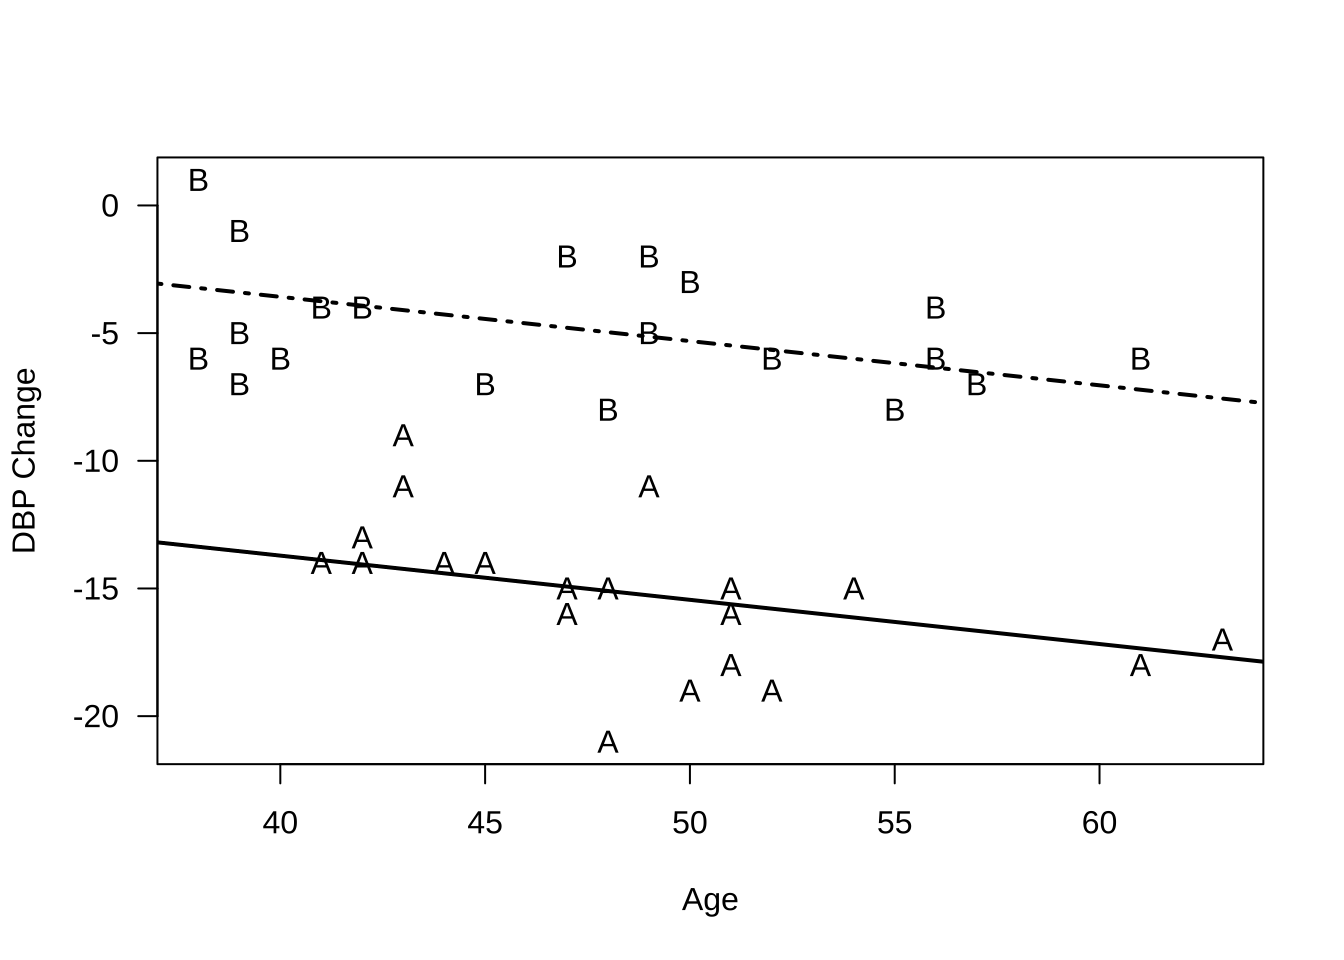
\includegraphics{survival_files/figure-latex/unnamed-chunk-10-1.pdf}

\hypertarget{uxc911uxc704-uxc0dduxc874uxc2dcuxac04}{%
\section{중위 생존시간}\label{uxc911uxc704-uxc0dduxc874uxc2dcuxac04}}

중위 생존시간의 추정량은 \(\hat t_{med}\) 다음 방정식을 만족하는 \(t\)의 값이다.

\[ \hat t_{med} = \inf ~ \{t~|~ \hat S(t) \le 1/2 \} \]

\begin{Shaded}
\begin{Highlighting}[]
\NormalTok{res.km}
\end{Highlighting}
\end{Shaded}

\begin{verbatim}
## Call: survfit(formula = Surv(t, cens) ~ 1, conf.type = "log-log")
## 
##       n  events  median 0.95LCL 0.95UCL 
##      11       7      31      13      NA
\end{verbatim}

\hypertarget{uxd655uxb960-uxacfcuxc815uxacfc-nelson-aalen-uxcd94uxc815uxb7c9}{%
\section{확률 과정과 Nelson-Aalen 추정량}\label{uxd655uxb960-uxacfcuxc815uxacfc-nelson-aalen-uxcd94uxc815uxb7c9}}

이제 위험함수를 추정하는 Nelson-Aalen 추정량을 확률 과정으로 유도해보자.

먼저 생존시간 \(T_i\)에 대한 계수과정(counting process) \(Y_i(t)\) 을 정의해 보자.
\(Y_i(t)\) 는 사건이 일어나기 전 까지 1인 함수이며 시간 \(t\) 까지 \(i\) 번째 개체가 위험 그룹(at risk at \(t\))에 속한는 지를 나타내는 확률과정이다.

\[ Y_i(t) = I(T_i \ge t)\]

또 하나의 계수과정 \(N_i(t)\)를 아래와 같이 정의한다. \(N_i(t)\) 는 절단이 없는 자 개체에 대하여 시간 \(t\) 까지 사건이 일어났는지를 알려주는 과정이다.

\[ N_i(t) = I(T_i \le t, \delta_i=1) \]

\(Y_i(t)\) 와 \(N_i(t)\)는 다음과 같은 모양을 가진 시간에 대한 함수이다.

\begin{figure}
\centering
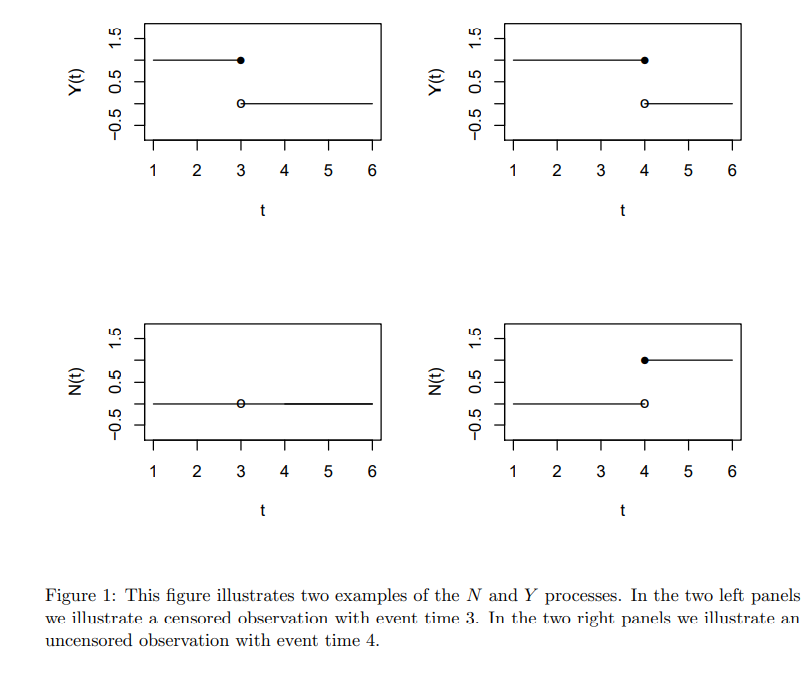
\includegraphics{images/process.PNG}
\caption{\(Y_i(t)\) 와 \(N_i(t)\)}
\end{figure}

\begin{itemize}
\tightlist
\item
  \(Y_i(t)\)는 왼쪽 연속함수(left continuity)의 형태를 가진다. 오른쪽 연속인 확률과정을 예측가능한 과정(predictable process) 라고 한다.
\item
  \(N_i(t)\)는 오른쪽 연속함수(right continuity)의 형태를 가진다.
\end{itemize}

이제 두 확률 과정의 합을 정의하자.

\[ \bar Y(t) =\sum_{t_i \le t} Y_i(t)  \quad \text{  number at risk at } t\]

\[ \bar N(t) =\sum_{t_i \le t} N_i(t)  \quad \text{  number of failures up to} t\]

이제 누적 위험함수는 매우 짧은 시간 \(h\) 에 대하녀 다음과 같은 근사식이 성립한다.

\[ H(s+h) - H(s) \approx h(s) h \]

위의 식에서 \(h(s)h\) 는 시간 \([s, s+h]\) 동안에 일어난 사건의 발생률이라고 볼 수 있다. 따라서 \(h(s)h\) 는 시간 \([s, s+h]\) 동안에 일어난 사건의 발생한 사건의
수 \(\bar N(s+h) -\bar N(s)\)를 시간 \(s\) 에 위험해 처한 개채의 수 \(\bar Y(s)\) 로 나는 값으로 추정할 수 있다.

이러한 사실을 이용하면 다음과 같은 추정식을 얻는다.

\[ \hat H(t) = \int_0^t \frac{d \bar N(s)} {\bar Y(s)} \]

위에서 구한 추정량 \(\hat H(t)\) 는 각 사건이 일어날 경우만 점프가 생기므로 다음과 같이 쓸수 있다.

\[ \hat H(t)  =\sum_{t_i \le t} \frac{\Delta \bar N(t_i)}{\bar Y(ti)}  =  \sum_{t_i \le t} \frac{d_i}{n_i}\]

\begin{Shaded}
\begin{Highlighting}[]
\FunctionTok{plot}\NormalTok{(res.fh, }\AttributeTok{cumhaz=}\ConstantTok{TRUE}\NormalTok{)}
\end{Highlighting}
\end{Shaded}

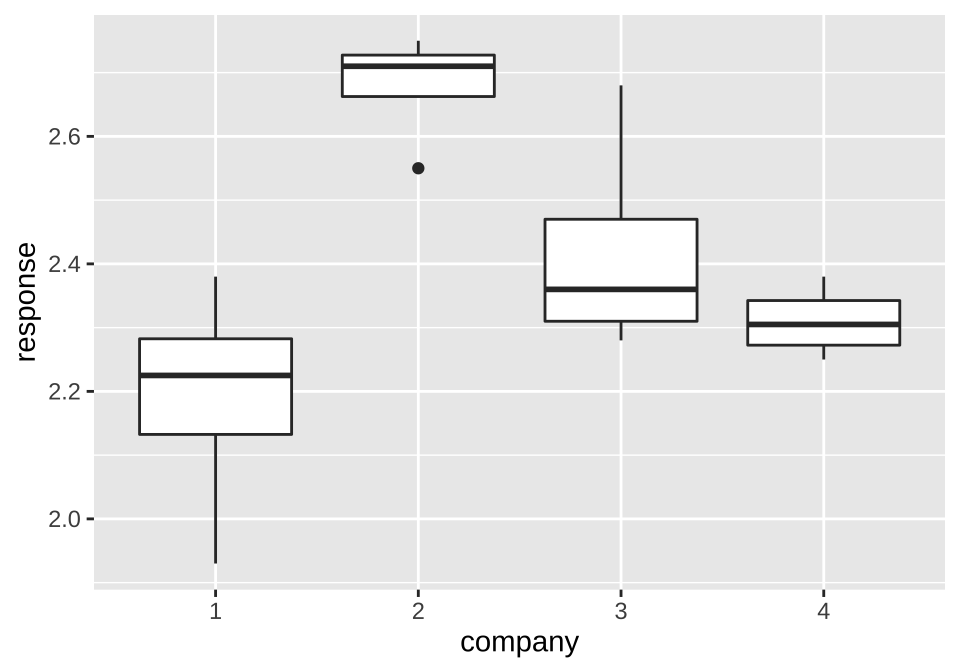
\includegraphics{survival_files/figure-latex/unnamed-chunk-12-1.pdf}

\hypertarget{uxc608uxc81c}{%
\section{예제}\label{uxc608uxc81c}}

clinical trial of the chemotherapeutic agent Xelox administered to patients with advanced gastric cancer prior to surgery. The primary outcome of interest is ``progression-free survival.'' This quantity is defined as the time from entry into a clinical trial until progression or death, whichever comes first.

\begin{Shaded}
\begin{Highlighting}[]
\NormalTok{timeMonths }\OtherTok{\textless{}{-}}\NormalTok{ gastricXelox}\SpecialCharTok{$}\NormalTok{timeWeeks}\SpecialCharTok{*}\DecValTok{7}\SpecialCharTok{/}\FloatTok{30.25}
\NormalTok{result.km }\OtherTok{\textless{}{-}} \FunctionTok{survfit}\NormalTok{(}\FunctionTok{Surv}\NormalTok{(timeMonths, delta) }\SpecialCharTok{\textasciitilde{}} \DecValTok{1}\NormalTok{, }\AttributeTok{conf.type=}\StringTok{"log{-}log"}\NormalTok{, }\AttributeTok{data=}\NormalTok{gastricXelox)}
\CommentTok{\# median survival and 95\% confidence interval is printed as follows:}
\NormalTok{result.km}
\end{Highlighting}
\end{Shaded}

\begin{verbatim}
## Call: survfit(formula = Surv(timeMonths, delta) ~ 1, data = gastricXelox, 
##     conf.type = "log-log")
## 
##       n  events  median 0.95LCL 0.95UCL 
##   48.00   32.00   10.30    5.79   15.27
\end{verbatim}

\begin{Shaded}
\begin{Highlighting}[]
\FunctionTok{plot}\NormalTok{(result.km, }\AttributeTok{mark=}\StringTok{"|"}\NormalTok{, }\AttributeTok{ylab=}\StringTok{"Survival probability"}\NormalTok{, }\AttributeTok{xlab=}\StringTok{"Time in months"}\NormalTok{,}
     \AttributeTok{cex.axis=}\FloatTok{1.5}\NormalTok{, }\AttributeTok{cex.lab=}\FloatTok{1.5}\NormalTok{, }\AttributeTok{lwd=}\FloatTok{1.5}\NormalTok{)}
\end{Highlighting}
\end{Shaded}

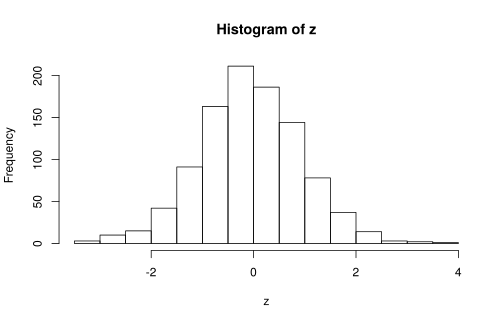
\includegraphics{survival_files/figure-latex/unnamed-chunk-13-1.pdf}

\begin{Shaded}
\begin{Highlighting}[]
\FunctionTok{plot}\NormalTok{(result.km, }\AttributeTok{cumhaz=}\ConstantTok{TRUE}\NormalTok{, }\AttributeTok{mark=}\StringTok{"|"}\NormalTok{, }\AttributeTok{ylab=}\StringTok{"cumulative hazrd"}\NormalTok{, }\AttributeTok{xlab=}\StringTok{"Time in months"}\NormalTok{,  }\AttributeTok{cex.axis=}\FloatTok{1.5}\NormalTok{, }\AttributeTok{cex.lab=}\FloatTok{1.5}\NormalTok{, }\AttributeTok{lwd=}\FloatTok{1.5}\NormalTok{)}
\end{Highlighting}
\end{Shaded}

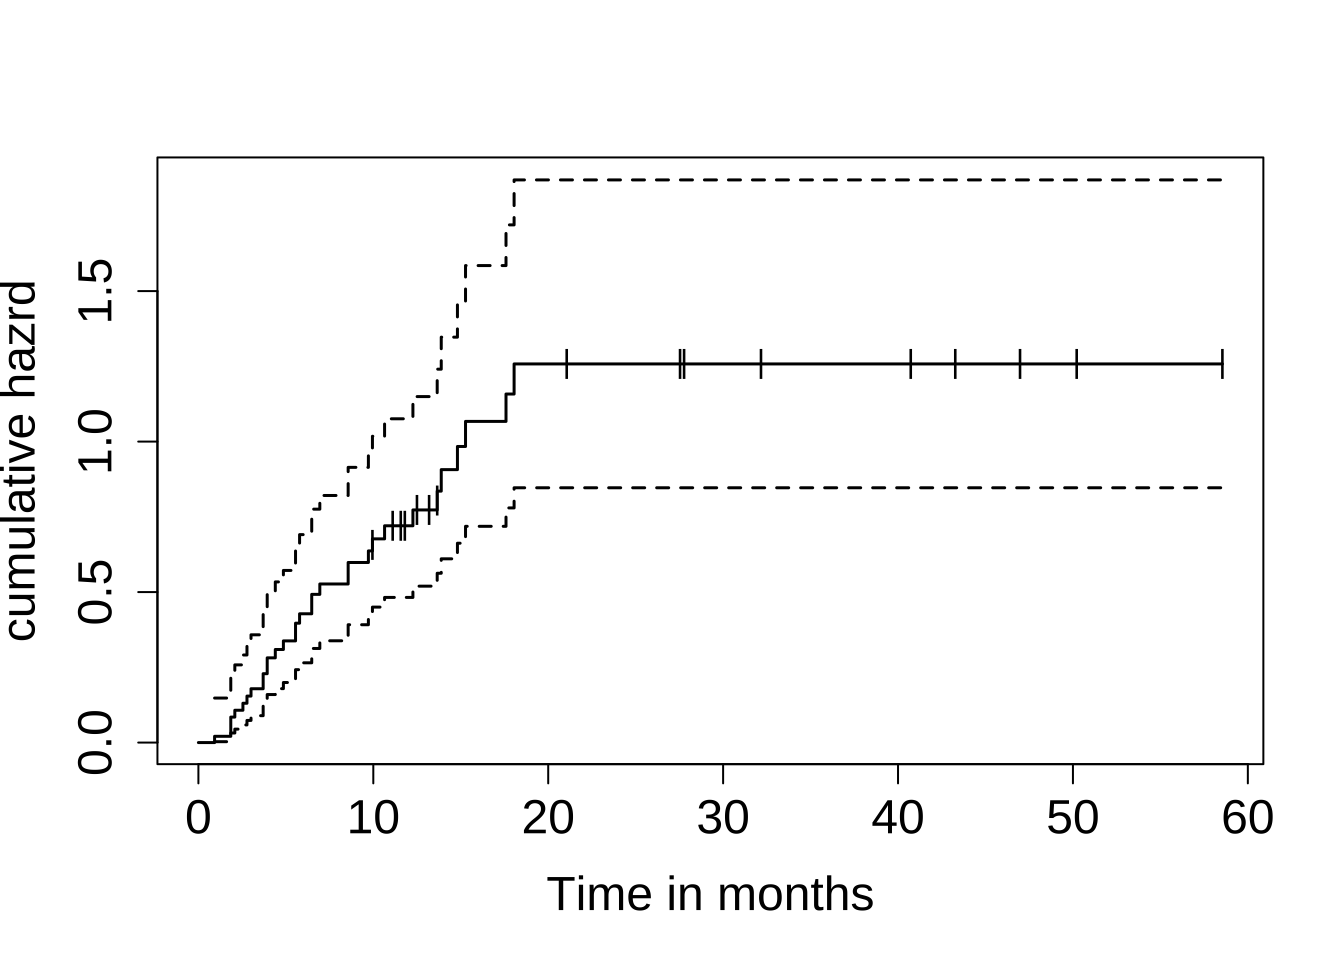
\includegraphics{survival_files/figure-latex/unnamed-chunk-13-2.pdf}

\hypertarget{logrank}{%
\chapter{비모수적 방법을 이용한 생존함수의 비교}\label{logrank}}

\hypertarget{uxbe44uxbaa8uxc218uxc801-uxbc29uxbc95uxc744-uxc774uxc6a9uxd55c-uxc0dduxc874uxd568uxc218uxc758-uxbe44uxad50}{%
\section{비모수적 방법을 이용한 생존함수의 비교}\label{uxbe44uxbaa8uxc218uxc801-uxbc29uxbc95uxc744-uxc774uxc6a9uxd55c-uxc0dduxc874uxd568uxc218uxc758-uxbe44uxad50}}

두 개의 독립 집단에 대하여 다음과 같이 생존시간을 관측하였다고 하자.

\begin{align*}
\text{group 1} \quad & (X_{11}, \delta_{11}), (X_{12}, \delta_{12}) , \dots ,(X_{1 n_1}, \delta_{1 n_1}) \\
\text{group 2} \quad & (X_{21}, \delta_{21}), (X_{22}, \delta_{22}) , \dots ,(X_{2 n_2}, \delta_{2 n_2}) \\
\end{align*}

두 개의 집단에 대한 생존함수가 동일하다는 다음 가설을 고려하자.

\[ H_0: S_1 = S_2 \quad H_1: S_1 \ne S_2  \]

위의 가설은 두 집단의 생존시간을 모두 합쳐서 순서대로 나열하고 중도절단이 없는 자료들에서 다음과 같은 \(2\times 2\) 분할표를 작성한 다음 CMH-검정 통계량을 이용하여 검정할 수 있다.

\begin{longtable}[]{@{}cccc@{}}
\toprule
처리/반응여부 & 사망 & 생존 & 합계\tabularnewline
\midrule
\endhead
1 & \(a\) & \(b\) & \(n_1\)\tabularnewline
2 & \(c\) & \(d\) & \(n_2\)\tabularnewline
합계 & \(m_1\) & \(m_2\) & \(n\)\tabularnewline
\bottomrule
\end{longtable}

다음과 같은 예제 자료를 고려해보자

\begin{align*}
\text{[group 1]} \quad & 3,~~5,~~7,~~9+~~, 18 \\
\text{[group 2]} \quad & 12,~~ 19,~~ 20,~~ 20+,~~ 33+ \\
\end{align*}

두 표본을 합쳐서 순서대로 놓으면 다음과 같다.

\[ 3,~~5,~~7,~~9+~~12,~~ 18, ~~ 19,~~ 20,~~ 20+,~~ 33+  \]

이제 중도절단이 없는 자료들(\(3,5,7,12,18,19,20\))에 대하여 각각 \(2\times 2\) 분할표를 작성하고 CMH-검정 통계량을 계산할 수 있다. 각 분할표와 관련 통계량을 다음과 같은 표로 정리할 수 있다.

\begin{longtable}[]{@{}ccccccccc@{}}
\toprule
\(X\) & \(n\) & \(m_1\) & \(n_1\) & \(a\) & \(E_0(A)\) & \(a-E_0(A)\) & \(m_1 m_2/(n-1)\) & \(n_1 n_2 /n^2\)\tabularnewline
\midrule
\endhead
3 & 10 & 1 & 5 & 1 & 0.50 & 0.50 & 1 & 0.2500\tabularnewline
5 & 9 & 1 & 4 & 1 & 0.44 & 0.56 & 1 & 0.2469\tabularnewline
7 & 8 & 1 & 3 & 1 & 0.38 & 0.62 & 1 & 0.2344\tabularnewline
12 & 6 & 1 & 1 & 0 & 0.17 & -0.17 & 1 & 0.1389\tabularnewline
18 & 5 & 1 & 1 & 1 & 0.20 & 0.80 & 1 & 0.1600\tabularnewline
19 & 4 & 1 & 0 & 0 & 0 & 0 & 1 & 0\tabularnewline
20 & 3 & 1 & 0 & 0 & 0 & 0 & 1 & 0\tabularnewline
\bottomrule
\end{longtable}

이제 다음과 같이 CMH 통계량을 계산할 수 있다.

\[ CMH ~~\chi^2 = \frac {[ \sum (a-E_0(A))]^2}{ \sum [m_1 m_2/(n-1)][n_1 n_2 /n^2] }  \]

여기서

\begin{align*}
\sum (a-E_0(A)) & = 0.50 + 0.56 + 0.62 -0.17 + 0.80 \\
& = 2.31 \\
 \sum [m_1 m_2/(n-1)][n_1 n_2 /n^2] & = (1)(0.2500) + (1)(0.2469) + (1)(0.2344)  \\
 &+ (1)(0.1389) + (1)(0.1600) + (1)(0) + (1)(0) \\
 & = 1.0302
\end{align*}

따라서
\[ CMH ~~\chi^2 = \frac{(2.31)^2} {1.0302}  = 5.1796   \]

유의수준 \(\alpha=0.05\)에서 \(\chi^2(1,0.95) = 3.84159 <5.1796\)이므로 \(H_0\)를 기각한다. 즉 두 집단의 생존함수는 같지 않다.

\begin{Shaded}
\begin{Highlighting}[]
\NormalTok{t }\OtherTok{\textless{}{-}} \FunctionTok{c}\NormalTok{(}\DecValTok{3}\NormalTok{, }\DecValTok{5}\NormalTok{, }\DecValTok{7}\NormalTok{, }\DecValTok{9}\NormalTok{, }\DecValTok{12}\NormalTok{,  }\DecValTok{18}\NormalTok{,   }\DecValTok{19}\NormalTok{,  }\DecValTok{20}\NormalTok{,  }\DecValTok{20}\NormalTok{,  }\DecValTok{33}\NormalTok{)}
\NormalTok{delta }\OtherTok{\textless{}{-}} \FunctionTok{c}\NormalTok{(}\DecValTok{1}\NormalTok{,}\DecValTok{1}\NormalTok{,}\DecValTok{1}\NormalTok{,}\DecValTok{0}\NormalTok{,}\DecValTok{1}\NormalTok{,}\DecValTok{1}\NormalTok{,}\DecValTok{1}\NormalTok{,}\DecValTok{1}\NormalTok{,}\DecValTok{0}\NormalTok{,}\DecValTok{0}\NormalTok{)}
\NormalTok{treat }\OtherTok{\textless{}{-}} \FunctionTok{c}\NormalTok{(}\StringTok{"A"}\NormalTok{, }\StringTok{"A"}\NormalTok{, }\StringTok{"A"}\NormalTok{, }\StringTok{"A"}\NormalTok{, }\StringTok{"B"}\NormalTok{, }\StringTok{"A"}\NormalTok{, }\StringTok{"B"}\NormalTok{, }\StringTok{"B"}\NormalTok{, }\StringTok{"B"}\NormalTok{, }\StringTok{"B"}\NormalTok{)}
\NormalTok{df }\OtherTok{\textless{}{-}} \FunctionTok{data.frame}\NormalTok{(t, delta, treat)}
\NormalTok{res.comp }\OtherTok{\textless{}{-}} \FunctionTok{survdiff}\NormalTok{(}\FunctionTok{Surv}\NormalTok{(t, delta) }\SpecialCharTok{\textasciitilde{}}\NormalTok{ treat, }\AttributeTok{data=}\NormalTok{df)}
\end{Highlighting}
\end{Shaded}

\hypertarget{uxc608uxc81c-1}{%
\section{예제}\label{uxc608uxc81c-1}}

The data set ``pancreatic'' in the ``asaur'' package consists of pancreatic cancer data from a Phase II clinical trial where the primary outcome of interest is
progression-free survival. As we saw in the previous chapter, this quantity is defined
as the time from entry into a clinical trial until progression or death, whichever
comes first. The data consist of, for each patient, the stage, classified as ``LAPC''
(locally advanced pancreatic cancer) or ``MPC'' (metastatic pancreatic cancer), the
date of entry into the clinical trial, the date of death (all of the patients in this study
died), and the date of progression, if that was observed before death. The first six
observations are shown in this output.

\begin{Shaded}
\begin{Highlighting}[]
\FunctionTok{head}\NormalTok{(pancreatic)}
\end{Highlighting}
\end{Shaded}

\begin{verbatim}
##   stage    onstudy progression      death
## 1     M 12/16/2005    2/2/2006 10/19/2006
## 2     M   1/6/2006   2/26/2006  4/19/2006
## 3    LA   2/3/2006    8/2/2006  1/19/2007
## 4     M  3/30/2006           .  5/11/2006
## 5    LA  4/27/2006   3/11/2007  5/29/2007
## 6     M   5/7/2006   6/25/2006 10/11/2006
\end{verbatim}

\begin{Shaded}
\begin{Highlighting}[]
\FunctionTok{attach}\NormalTok{(pancreatic)     }\CommentTok{\# make the variable names accessible}

\CommentTok{\# convert the text dates into R dates}
\NormalTok{Progression.d }\OtherTok{\textless{}{-}} \FunctionTok{as.date}\NormalTok{(}\FunctionTok{as.character}\NormalTok{(progression))}
\NormalTok{OnStudy.d }\OtherTok{\textless{}{-}} \FunctionTok{as.date}\NormalTok{(}\FunctionTok{as.character}\NormalTok{(onstudy))}
\NormalTok{Death.d }\OtherTok{\textless{}{-}} \FunctionTok{as.date}\NormalTok{(}\FunctionTok{as.character}\NormalTok{(death))}

\CommentTok{\# compute progression{-}free survival}

\NormalTok{progressionOnly }\OtherTok{\textless{}{-}}\NormalTok{ Progression.d }\SpecialCharTok{{-}}\NormalTok{ OnStudy.d}
\NormalTok{overallSurvival }\OtherTok{\textless{}{-}}\NormalTok{ Death.d }\SpecialCharTok{{-}}\NormalTok{ OnStudy.d}
\NormalTok{pfs }\OtherTok{\textless{}{-}} \FunctionTok{pmin}\NormalTok{(progressionOnly, overallSurvival)}
\NormalTok{pfs[}\FunctionTok{is.na}\NormalTok{(pfs)] }\OtherTok{\textless{}{-}}\NormalTok{ overallSurvival[}\FunctionTok{is.na}\NormalTok{(pfs)]}

\CommentTok{\# convert pfs to months}

\NormalTok{os }\OtherTok{\textless{}{-}}\NormalTok{ overallSurvival}
\NormalTok{status }\OtherTok{\textless{}{-}} \FunctionTok{rep}\NormalTok{(}\DecValTok{1}\NormalTok{, }\FunctionTok{length}\NormalTok{(pfs))}

\CommentTok{\# Note:  "pancreatic2" is already part of the "asaur" package; this is how one would create it:}
\CommentTok{\#pancreatic2 \textless{}{-} data.frame(pfs, os, status, stage)    \# create "pancreatic2" data frame}

\CommentTok{\# library(pancreatic2) \# an alternative to the above is to just use pancreatic2}
\NormalTok{pfs.month }\OtherTok{\textless{}{-}}\NormalTok{ pfs}\SpecialCharTok{/}\FloatTok{30.5}

\FunctionTok{plot}\NormalTok{(}\FunctionTok{survfit}\NormalTok{(}\FunctionTok{Surv}\NormalTok{(pfs.month) }\SpecialCharTok{\textasciitilde{}}\NormalTok{ stage), }\AttributeTok{xlab=}\StringTok{"Time in months"}\NormalTok{,}
   \AttributeTok{ylab=}\StringTok{"Survival probability"}\NormalTok{, }\AttributeTok{col=}\FunctionTok{c}\NormalTok{(}\StringTok{"blue"}\NormalTok{, }\StringTok{"red"}\NormalTok{), }\AttributeTok{lwd=}\DecValTok{2}\NormalTok{)}
\FunctionTok{legend}\NormalTok{(}\StringTok{"topright"}\NormalTok{, }\AttributeTok{legend=}\FunctionTok{c}\NormalTok{(}\StringTok{"Locally advanced"}\NormalTok{, }\StringTok{"Metastatic"}\NormalTok{),}
  \AttributeTok{col=}\FunctionTok{c}\NormalTok{(}\StringTok{"blue"}\NormalTok{,}\StringTok{"red"}\NormalTok{), }\AttributeTok{lwd=}\DecValTok{2}\NormalTok{)}
\end{Highlighting}
\end{Shaded}

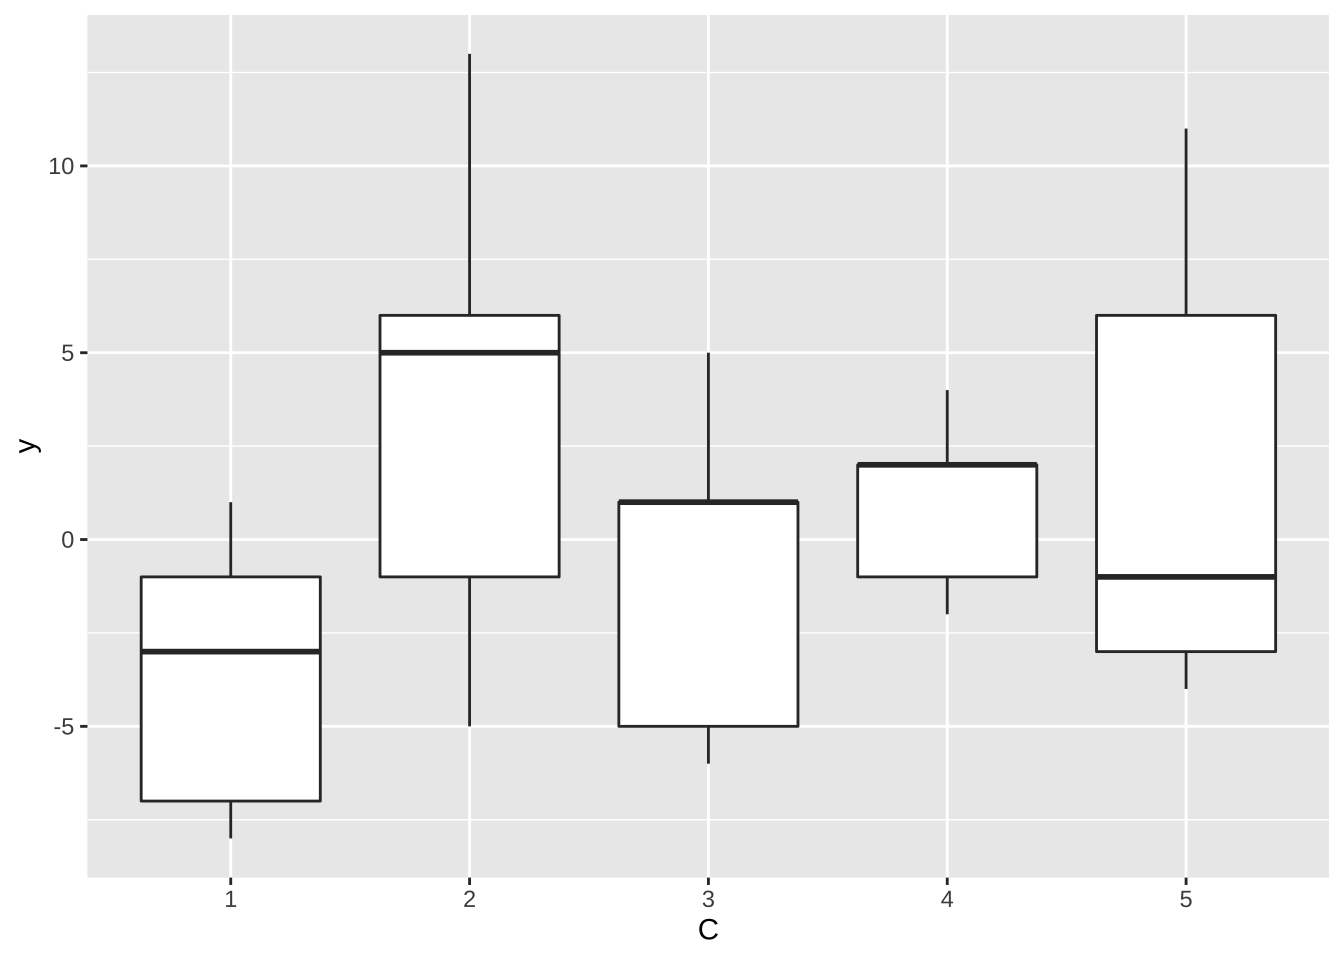
\includegraphics{survival_files/figure-latex/unnamed-chunk-15-1.pdf}

\hypertarget{uxc77cuxbc18uxd654-uxb85cuxadf8-uxc21cuxc704-uxac80uxc815}{%
\section{일반화 로그 순위 검정}\label{uxc77cuxbc18uxd654-uxb85cuxadf8-uxc21cuxc704-uxac80uxc815}}

\[ CMH ~~\chi^2 = \frac {w_i[ \sum (a-E_0(A))]^2}{ \sum w_i^2 [m_1 m_2/(n-1)][n_1 n_2 /n^2] }  \]

\hypertarget{appendix-appendix}{%
\appendix \addcontentsline{toc}{chapter}{\appendixname}}


\hypertarget{uxbd84uxd560uxd45c-uxac80uxc815}{%
\chapter{분할표 검정}\label{uxbd84uxd560uxd45c-uxac80uxc815}}

\hypertarget{times-2-uxbd84uxd560uxd45cuxc5d0uxc11c-uxb450-uxbe44uxc728uxc758-uxbe44uxad50}{%
\section{\texorpdfstring{\(2 \times 2\) 분할표에서 두 비율의 비교}{2 \textbackslash times 2 분할표에서 두 비율의 비교}}\label{times-2-uxbd84uxd560uxd45cuxc5d0uxc11c-uxb450-uxbe44uxc728uxc758-uxbe44uxad50}}

다음과 같은 \(2 \times 2\) 분할표에서 두 비율을 비교한다고 가정하자.

\begin{longtable}[]{@{}cccc@{}}
\toprule
처리/반응여부 & 반응 & 반응 안함 & 합계\tabularnewline
\midrule
\endhead
1 & \(a\) & \(b\) & \(n_1\)\tabularnewline
2 & \(c\) & \(d\) & \(n_2\)\tabularnewline
합계 & \(m_1\) & \(m_2\) & \(n\)\tabularnewline
\bottomrule
\end{longtable}

처리 1과 2가 서로 독립인 집단에 적용되었다면 두 집단의 반응 비율이 같다는 가설 \(H_0: p_1=p_2\)를 다음과 같은 통계량으로 검정할 수 있다.

\[ z = \frac{ \hat p_1 - \hat p_2} { \sqrt{\hat p (1-\hat p) (1/n_1 + 1/n_2)}} \]

위에서

\[ \hat p_1 = \frac{a}{n_1} \quad \hat p_2 = \frac{c}{n_2} \quad \hat p = \frac{m_1}{n} \]

\(n\)이 충분히 크면 귀무가설 하에서 통계량 \(z\)는 정규분포를 따르므로 \(|z|>z_{\alpha/2}\)이면 귀무가설을 기각한다.

카이제곱 분포의 정의에 의하여 통계량 \(z\)의 제곱 \(\chi^2 = z^2\)은 자유도가 1인 카이제곱분포를 따른다.

이때 통계량 \(z\)의 제곱은 \(2 \times 2\) 분할표에서 동일성 검정에 대한 카이제곱 통계량(교과서 46 페이지)과 동일하다.

\[ \chi^2 = z^2 = \frac {n(ad-bc)^2}{n_1 n_2 m_1 m_2} \]

만약에 귀무가설이 참이고 주변합 \(n_1, n_2, m_1, m_2\)가 고정되어 있다고 가정하면 첫번째 행, 첫번째 열의 값 \(A=a\)의 분포는 다음과 같은 초기하분포(Hypergeometric distribution)를 따른다.

\[ P(A=a) = \frac{ \binom{n_1}{a} \binom{n_2}{m_1-a} } {\binom{n}{m_1}} \]

위의 초기하분포에서 \(A=a\)의 기대값과 분산은 다음과 같다.

\[ E_0(A) = \frac{n_1 m_2}{n}, \quad Var_0 (A) = \frac{n_1 n_2 m_1 m_2}{n^2(n-1)} \]

따라서 다음이 성립하며

\[ ad-bc = n[a-E_0(A)], \quad n_1 n_2 m_1 m_2 = n^2(n-1)  Var_0 (A)  \]

이제 \(2 \times 2\) 분할표에서 동일성 검정에 대한 카이제곱 통계량은 초기하분포와 다음과 같은 관계를 가진다.

\[ \chi^2 = z^2 = \frac {n(ad-bc)^2}{n_1 n_2 m_1 m_2} = \frac{n}{n-1} \left [ \frac{a-E_0(A)}{\sqrt{var_0(A)}} \right ]^2 \]

\hypertarget{uxcf54uxd06cuxb780-uxb9e8uxd154-uxd578uxc824-uxac80uxc815}{%
\section{코크란-맨텔-핸젤 검정}\label{uxcf54uxd06cuxb780-uxb9e8uxd154-uxd578uxc824-uxac80uxc815}}

\begin{itemize}
\tightlist
\item
  교과서 53-55 페이지 참조
\end{itemize}

전체 자료가 다음과 같이 \(K\) 개의 \(2 \times 2\) 분할표로 나누어 진다면

\begin{longtable}[]{@{}cccc@{}}
\toprule
처리/반응여부 & 반응 & 반응 안함 & 합계\tabularnewline
\midrule
\endhead
1 & \(n_{k11}\) & \(n_{k12}\) & \(n_{k1+}\)\tabularnewline
2 & \(n_{k21}\) & \(n_{k22}\) & \(n_{k2+}\)\tabularnewline
합계 & \(n_{k+1}\) & \(n_{k+2}\) & \(n_{k}\)\tabularnewline
\bottomrule
\end{longtable}

전체 자료에 대하여 처리의 반응률에 대한 다음과 같은 가설검정을

\[ H_0: p_{k1} = p_{k2}, ~~k=1,2,\dots,K \quad \text{vs.} \quad H_0: not~~ H_0 \]

다음과 같은 코크란-맨텔-핸젤 검정 통계량(CMH 검정 통계량)으로 검정할 수 있다.

\[ Q_{CMH} = \frac { [ \sum_{k=1}^ K n_{k11} - \sum_{k=1}^K E(n_{k11}|H_0)]^2} { \sum_{k=1}^K Var(n_{k11}|H_0)} \]

위의 통계량에서 각 \(2 \times 2\) 분할표에 대한 기대값과 분산은 다음과 같이 계산할 수 있다.

\[  E(n_{k11}|H_0) = \frac{n_{k1+} n_{k+1}}{n_k} \quad
Var(n_{k11}|H_0) = \frac{n_{k1+}n_{k2+} n_{k+1}n_{k+2}}{n^2_k(n_k-1)} \]

CMH 검정 통계량 \(Q_{CMH}\)은 귀무가설 \(H_0\)가 옳은 경우에 자유도 1을 가지는 카이제곱 분포를 따른다.

\backmatter

  \bibliography{reference.bib}

\end{document}
